\documentclass[letterpaper, reqno,11pt]{article}
\usepackage[margin=1.0in]{geometry}
\usepackage{color,latexsym,amsmath,amssymb,graphicx,float,listings,tikz}
\usepackage{hyperref}

\hypersetup{
colorlinks=true,
linkcolor=magenta,
filecolor=magenta,
urlcolor=cyan,
}

\graphicspath{ {images/} }

\begin{document}

\pagenumbering{arabic}


\begin{titlepage}
\newgeometry{margin=3cm}
\centering

\vspace*{\stretch{2}}

\Large ELEC 302 Lab 1 Report

\vspace{\stretch{1}}

\normalsize Power Supplies and Voltage Regulators

\vspace{\stretch{0.5}}

\begin{tabular}{ll}
Name & Xander Naumenko \\[2ex]
Student Number  & 38198354 \\[2ex]
Lab Group            & L2C \\[2ex]
Experiment Date            & 2023-02-05 \\[2ex]
Partner's Name &  Brian Sun
\end{tabular}

\vspace{\stretch{3}}


\vspace{\stretch{2}}
\end{titlepage}


\section{Task 1}

{\medskip\noindent\bf Part 1.} 

For part 1 we simply measured the waveform coming out of a transformer. The setup can seen in the left half of figure \ref{fig:t1}, before the diode and resistor were added. The resulting waveform can be seen in figure \ref{fig:t1p1}. From this we see the RMS voltage was $12$V.

\begin{figure}[htpb]
        \centering
        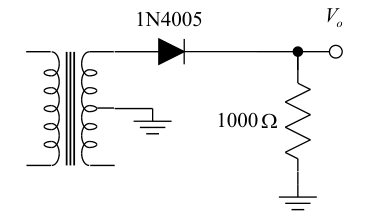
\includegraphics[width=0.5\textwidth]{t1}
        \caption{Setup for task 1. The first part of task 1 occured before the diode and resistor were added, and for the second part additional capacitors were added between $V_0$ and ground. Diagram taken from the lab manual.}
        \label{fig:t1}
\end{figure}

\begin{figure}[htpb]
        \centering
        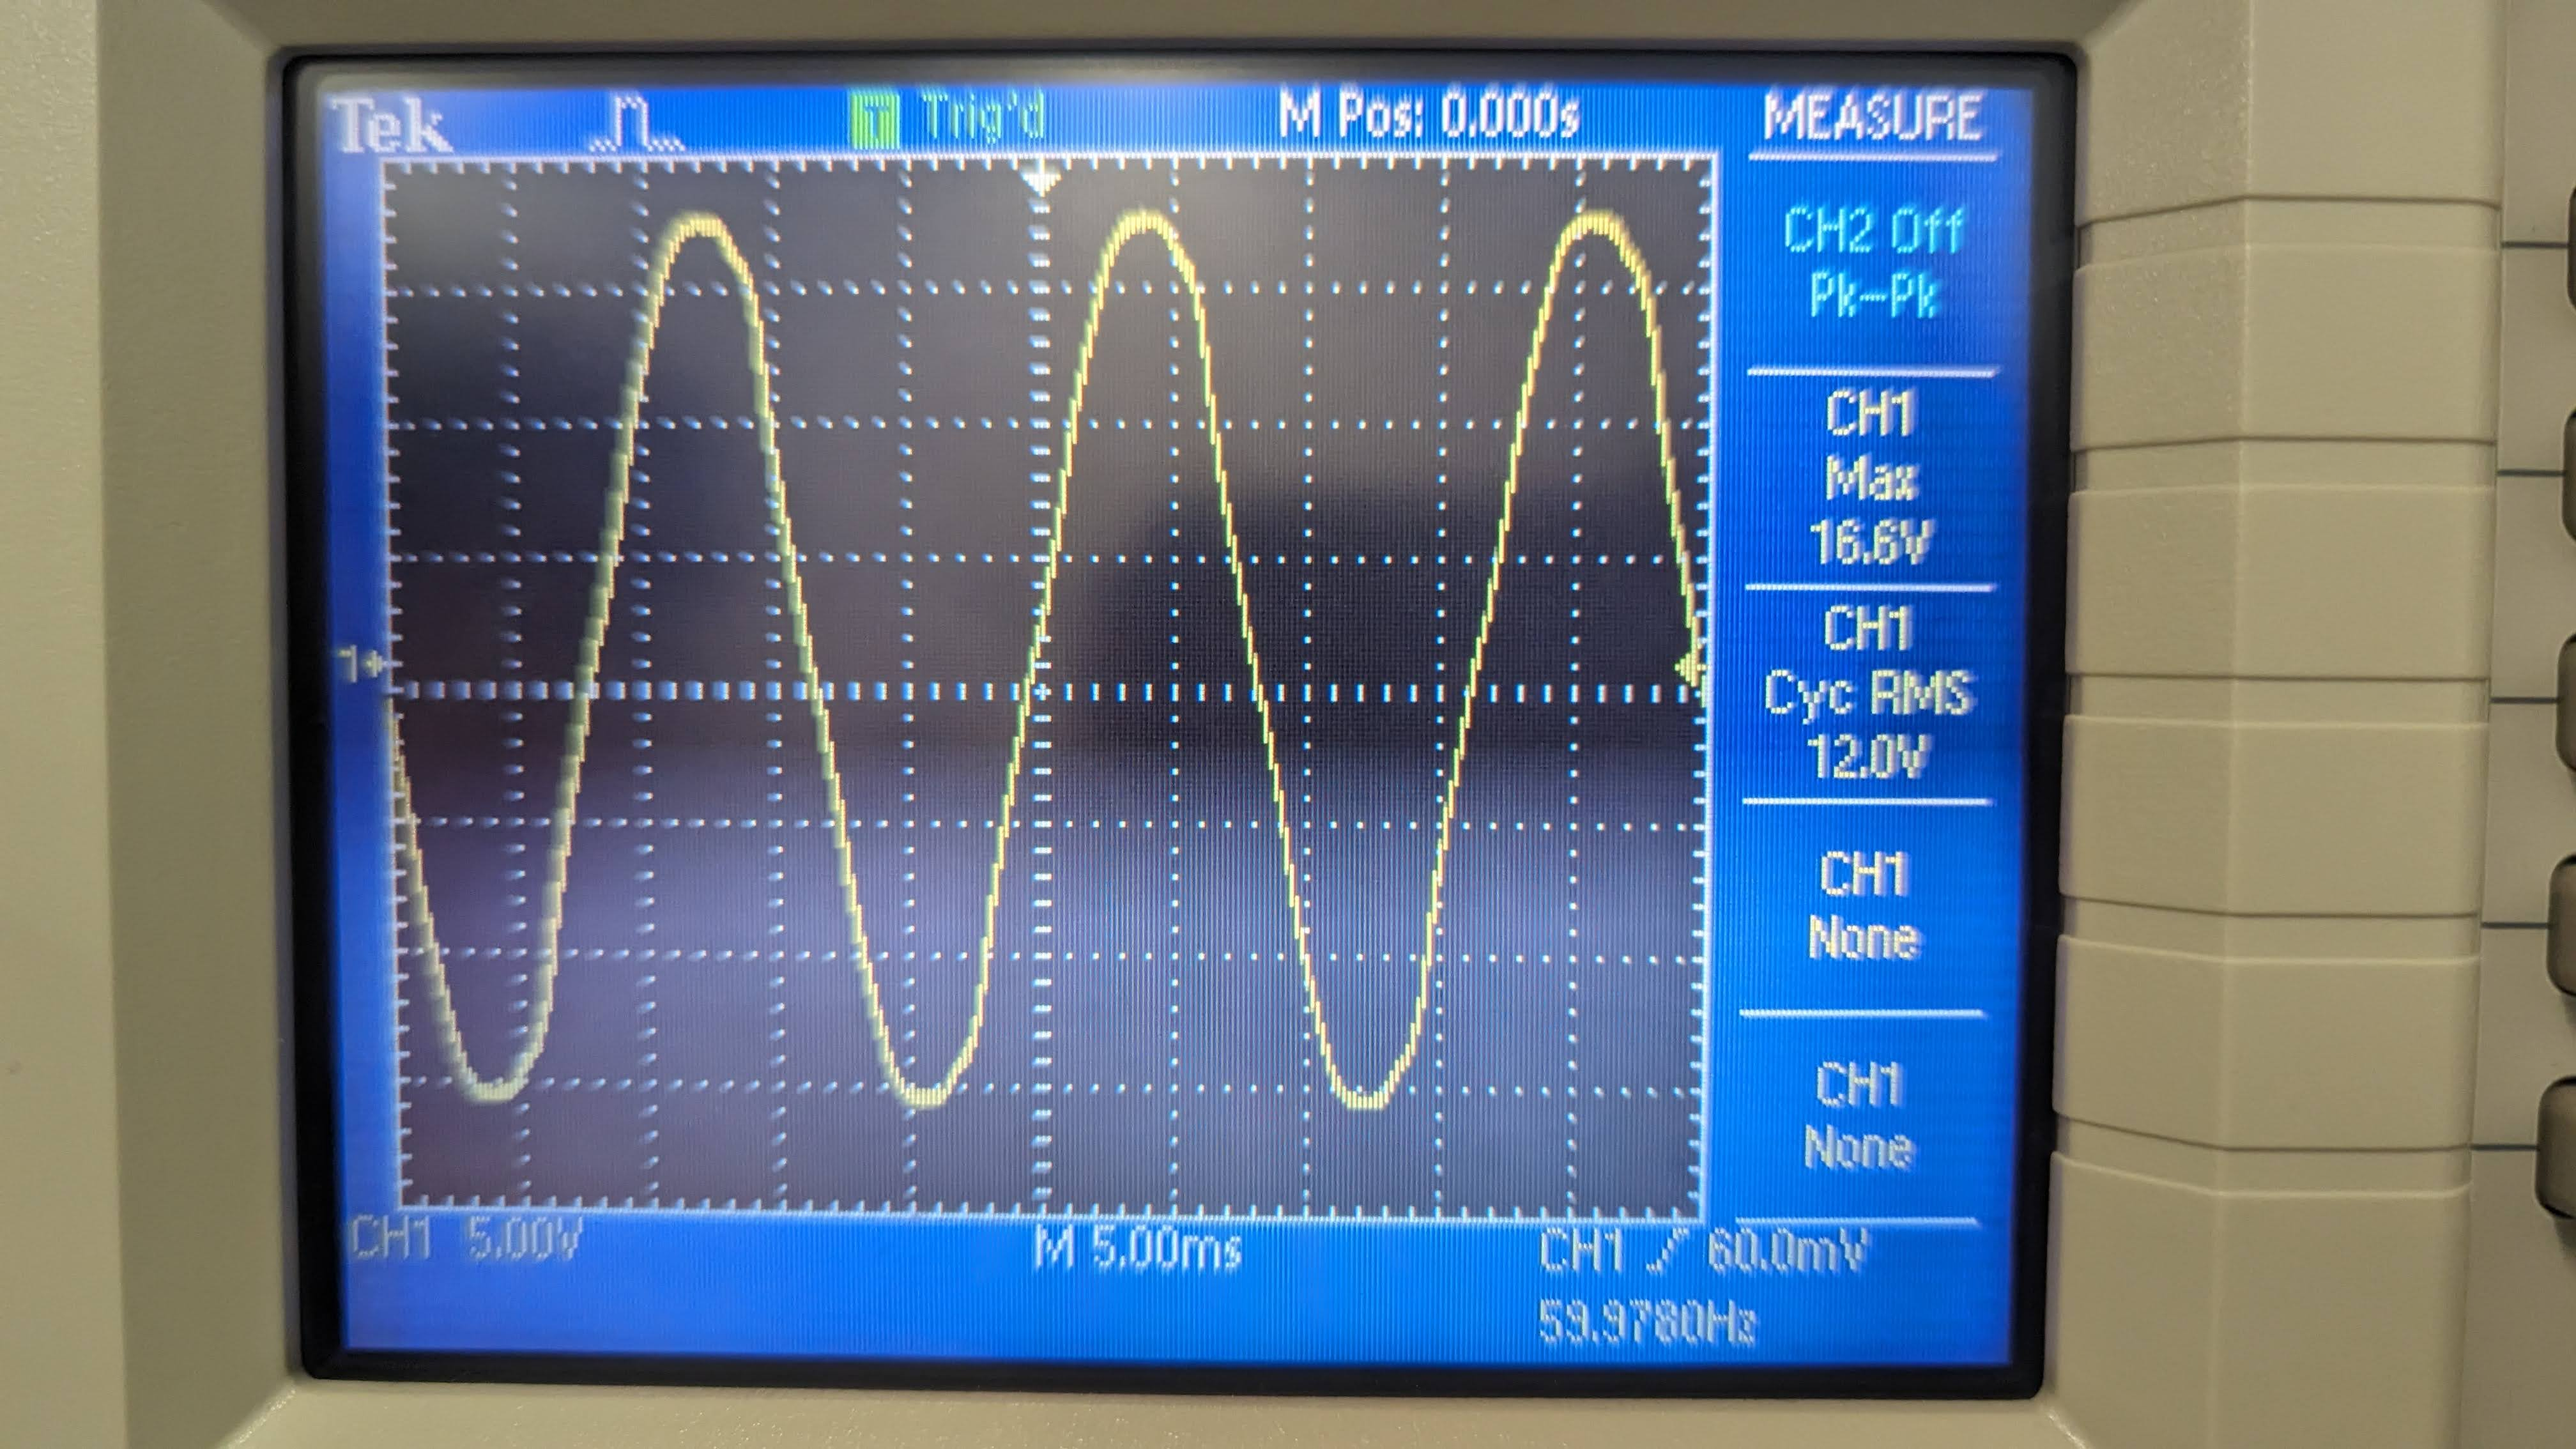
\includegraphics[width=0.8\textwidth]{lab1/t1p1}
        \caption{Task 1, part 1 waveform.}
        \label{fig:t1p1}
\end{figure}

{\medskip\noindent\bf Part 2.} In this section, we added the diode and resistor and measured the output voltage. The resulting waveform can be seen in figure \ref{fig:t1p2}. Before adding the capacitors, we see the peak voltage is $16$V. This is expected, since for a half wave rectifier the peak voltage is $V_p-V_d=16.6-0.6\approx 16$.

For the capacitor, we can use the formula given in class to calculate the value:
\[
C = \frac{V_p-V_d}{fR_LV_r}=\frac{16.8-0.7}{60\cdot 1000\cdot 1}=268.3\mu\text{F}
.\]
Since we don't have any capacitor values close to that, we instead used one 220$\mu$F and two $33\mu$F capacitors in parallel which has an equivalent capacitance of $286\mu$F. The resulting waveform can be seen in figure \ref{fig:t1p2}, the average DC output voltage is 15.3V, and as expected the ripple voltage is $920$mV which is just under the required $1$V.

\begin{figure}[htpb]
        \centering
        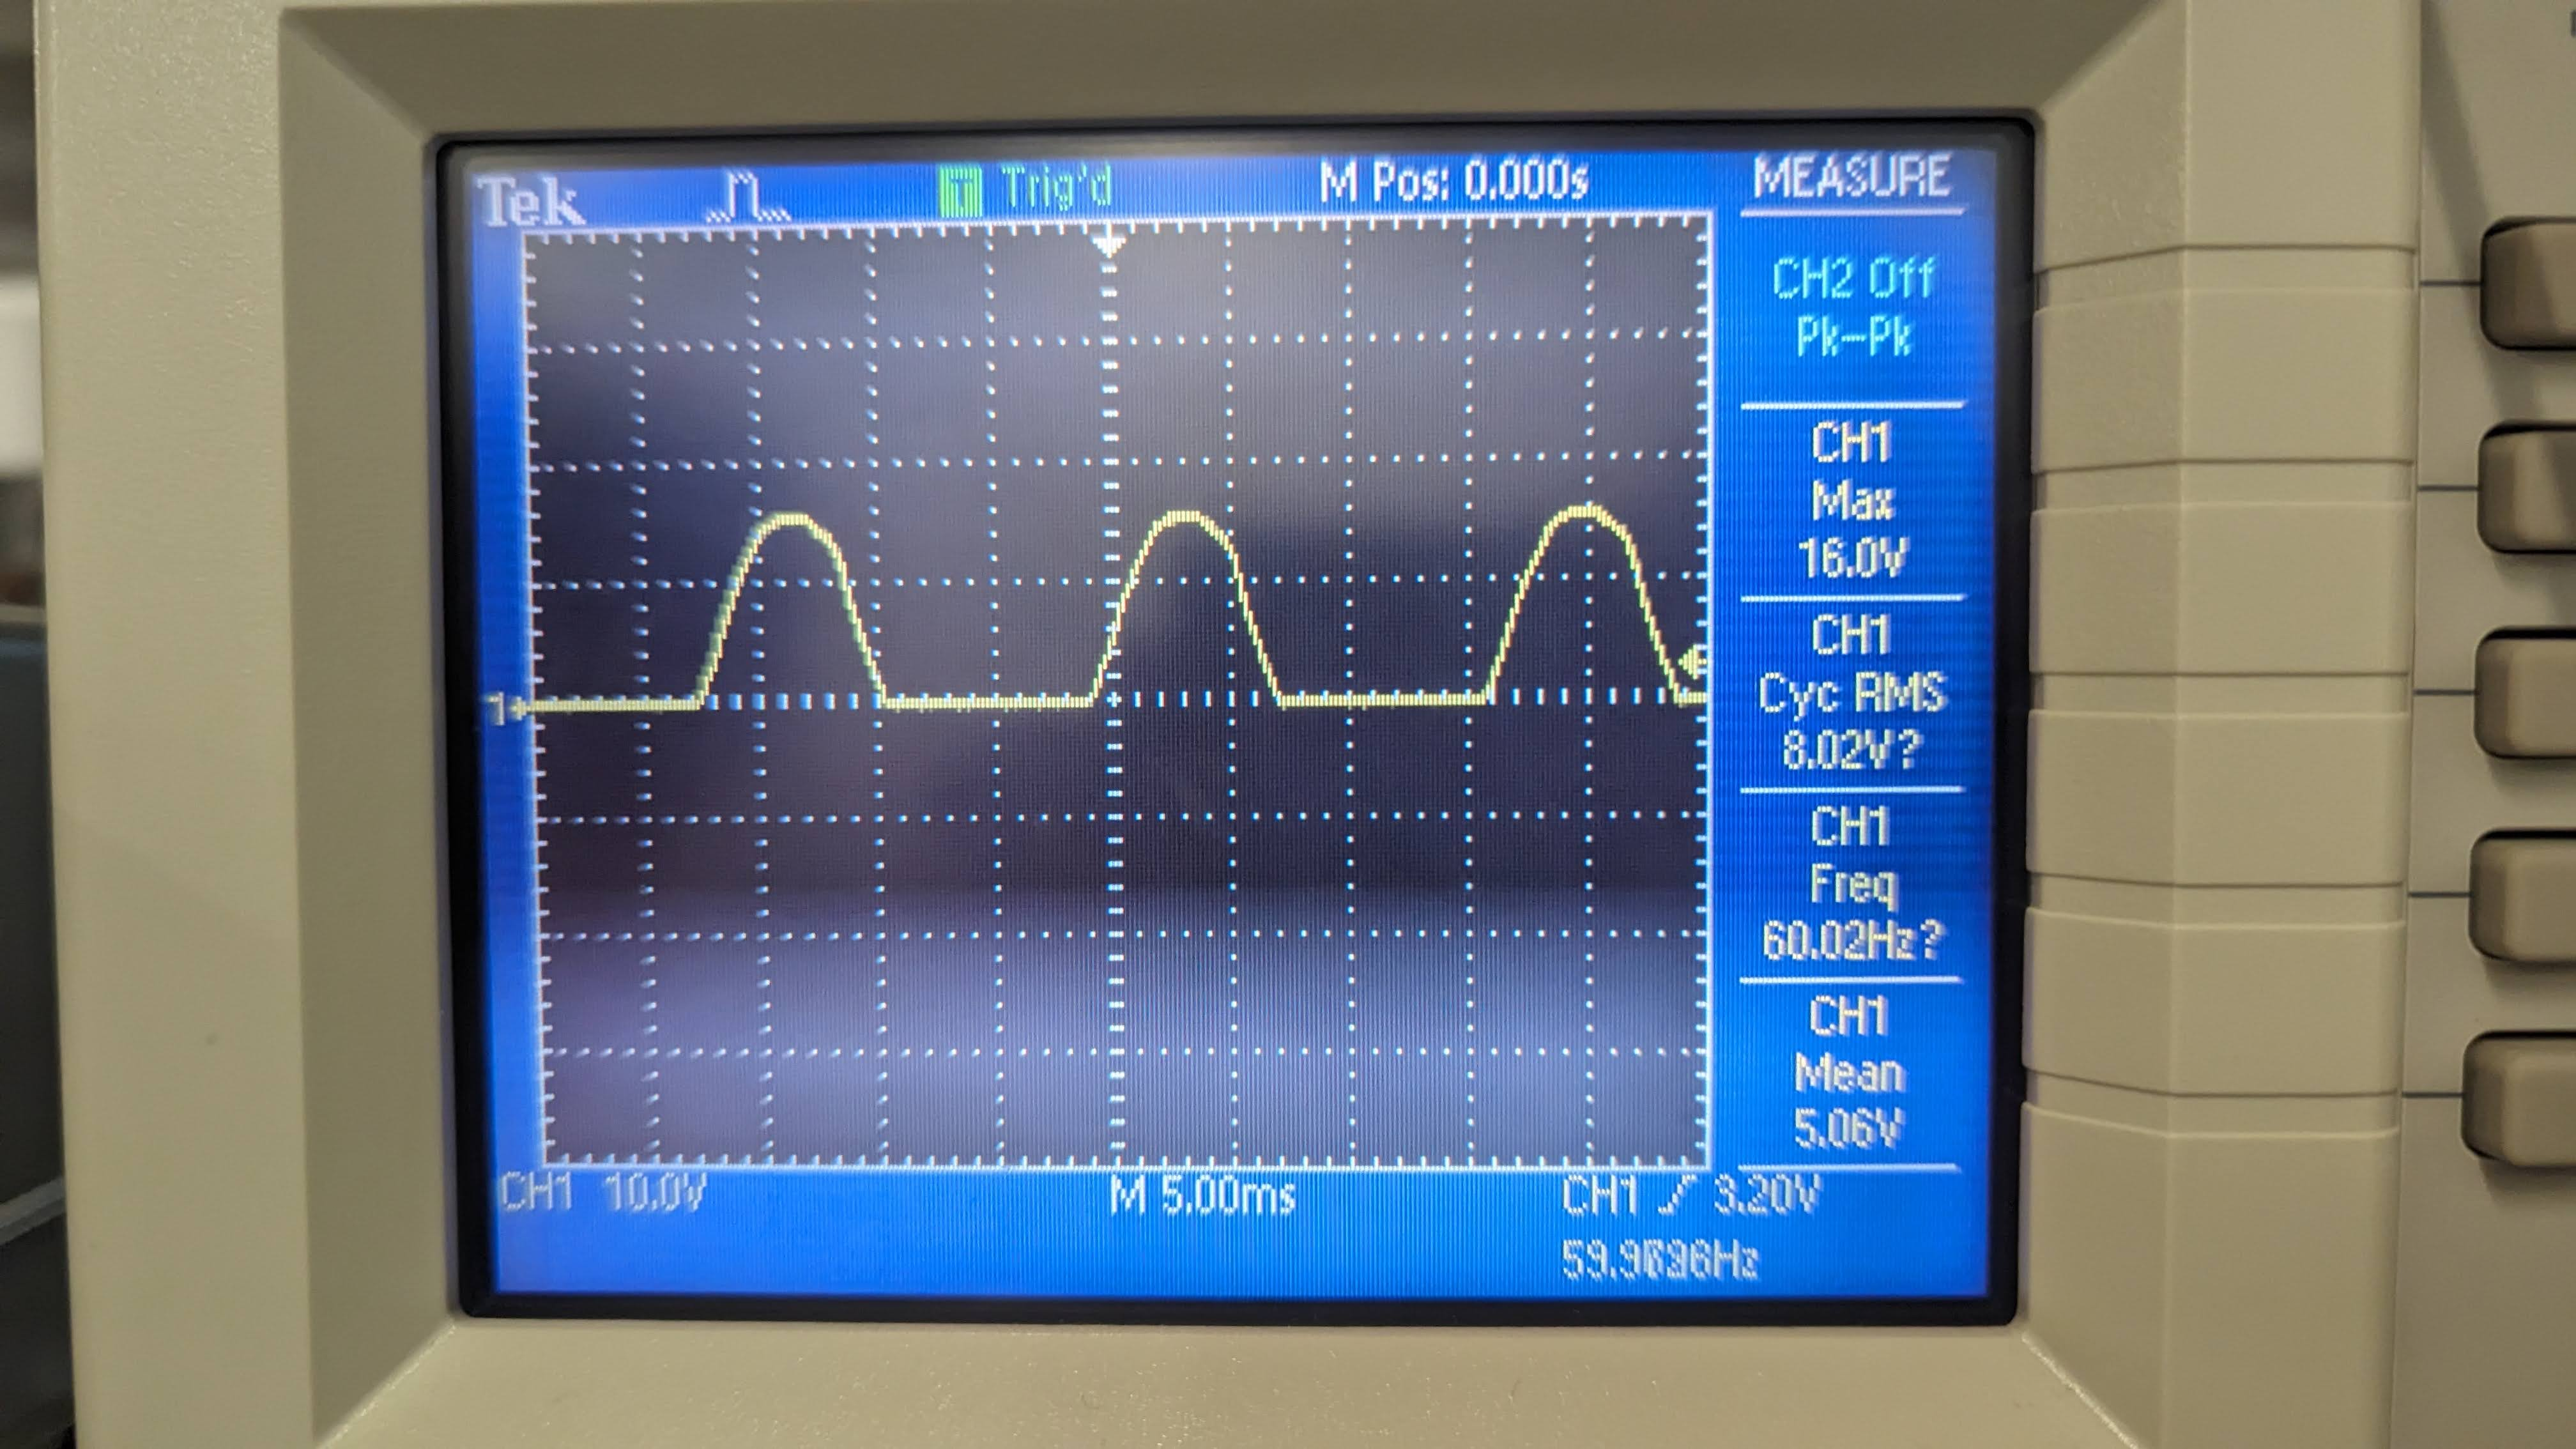
\includegraphics[width=0.45\textwidth]{lab1/t1p2b}
        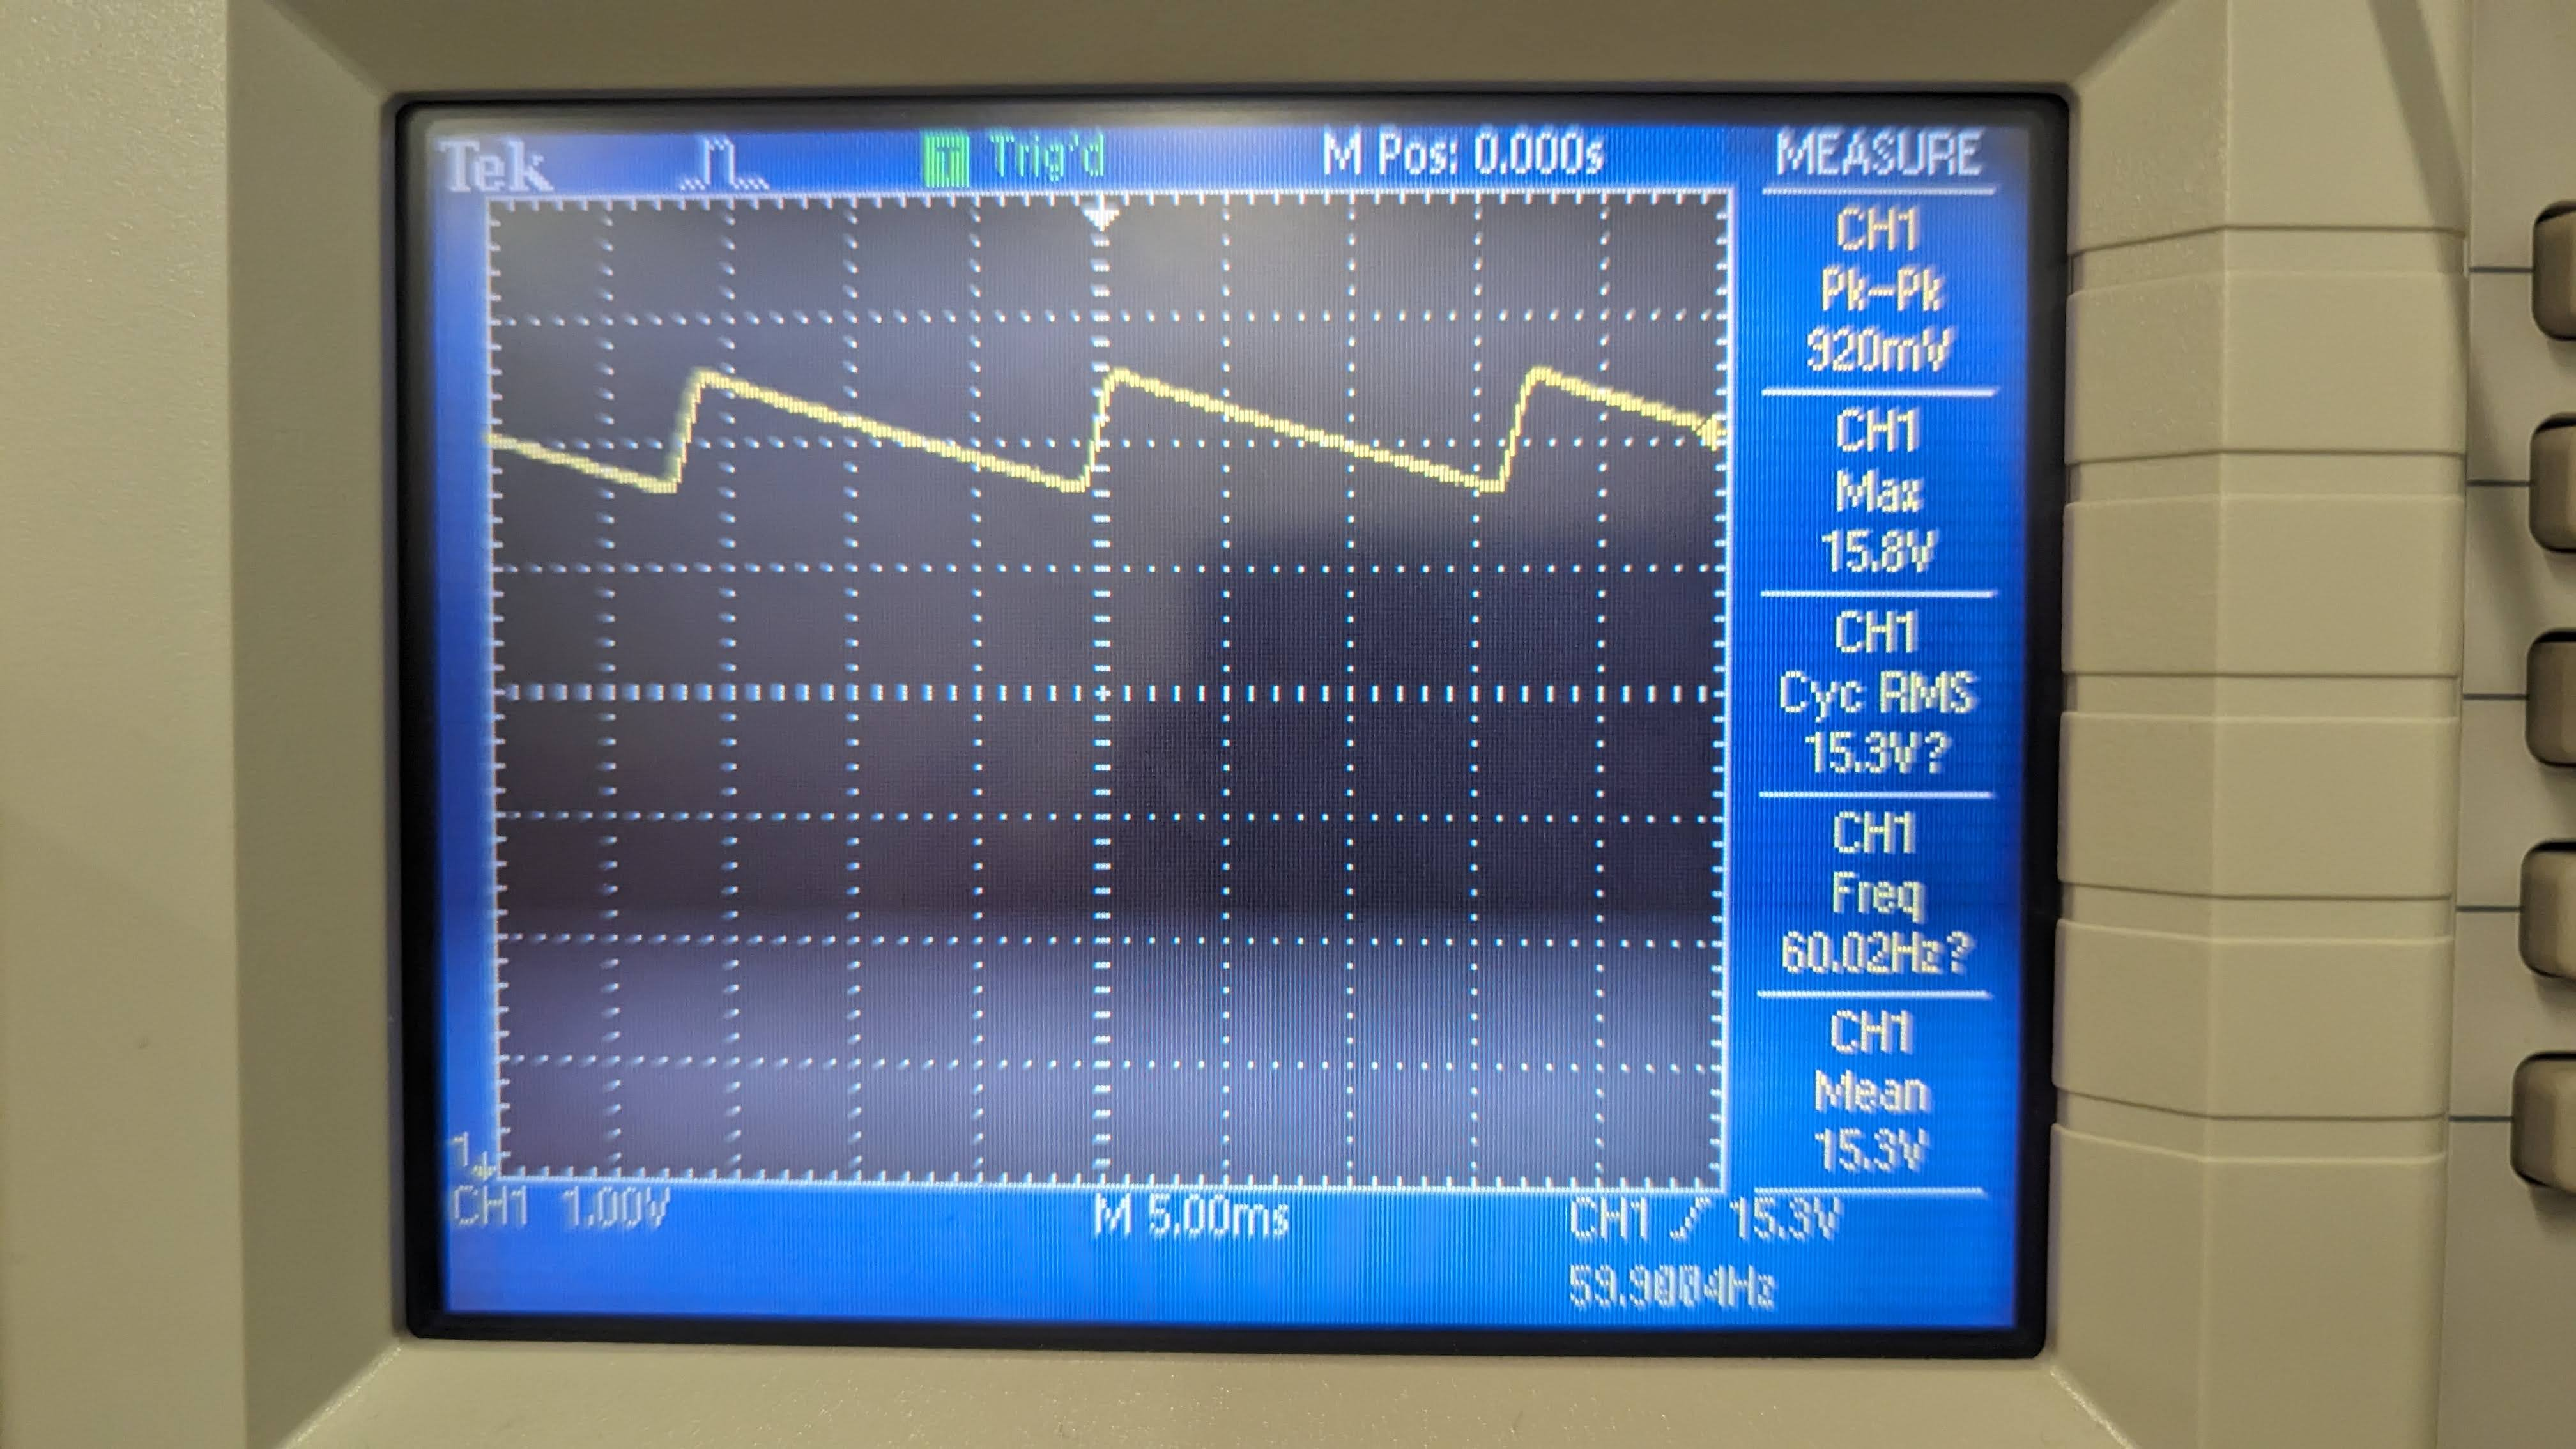
\includegraphics[width=0.45\textwidth]{lab1/t1p2c}
        \caption{Task 1, part 2 waveforms. The left is the $V_0$ without the capacitors, while the right is $V_0$ with capacitors, zoomed in to see the ripple. The ripple (i.e. Pk-Pk) can be seen to be $920$mV, less than the $1$V as required.}
        \label{fig:t1p2}
\end{figure}

\section{Task 2}

{\medskip\noindent\bf Part 1.} The setup can be seen in figure \ref{fig:t2a}.

\begin{figure}[htpb]
        \centering
        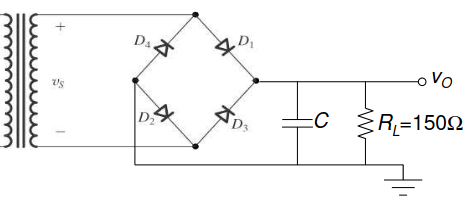
\includegraphics[width=0.5\textwidth]{t2a}
        \caption{Setup for task 2, part 1. Note that in our case $R_L=1\text{k}\Omega$, this diagram was taken from the lecture slides.}
        \label{fig:t2a}
\end{figure}

For the capacitor using the equation:
\[
C = \frac{V_p-2V_d}{2fR_LV_r}=\frac{33.2-1.4}{2\cdot 60\cdot 1000\cdot 1}=265\mu\text{F}
.\]
Again we used the same capacitor configuration as before of $286\mu$F since we didn't have a single capacitor of the correct value. The resulting waveforms can be seen in figure \ref{fig:t2p1}. The peak voltage before adding the capacitors was $31.2$V, while after adding them the average voltage was 30.6. This makes sense, as after adding the capacitor we'd expect the mean to be $V_p-\frac{V_r}{2}\approx 31.2-0.5\approx 31.6$. The ripple was $832$mV as expected.

Comparing with the previous part, the ripple was the same. Given the capacitors were specifically chosen to achieve the same target ripple though, this isn't too surprising. The output voltage for the bridge rectifier is twice as high for the same capacitors to achieve the same ripple though, which could make it a better fit for many applications.

\begin{figure}[htpb]
        \centering
        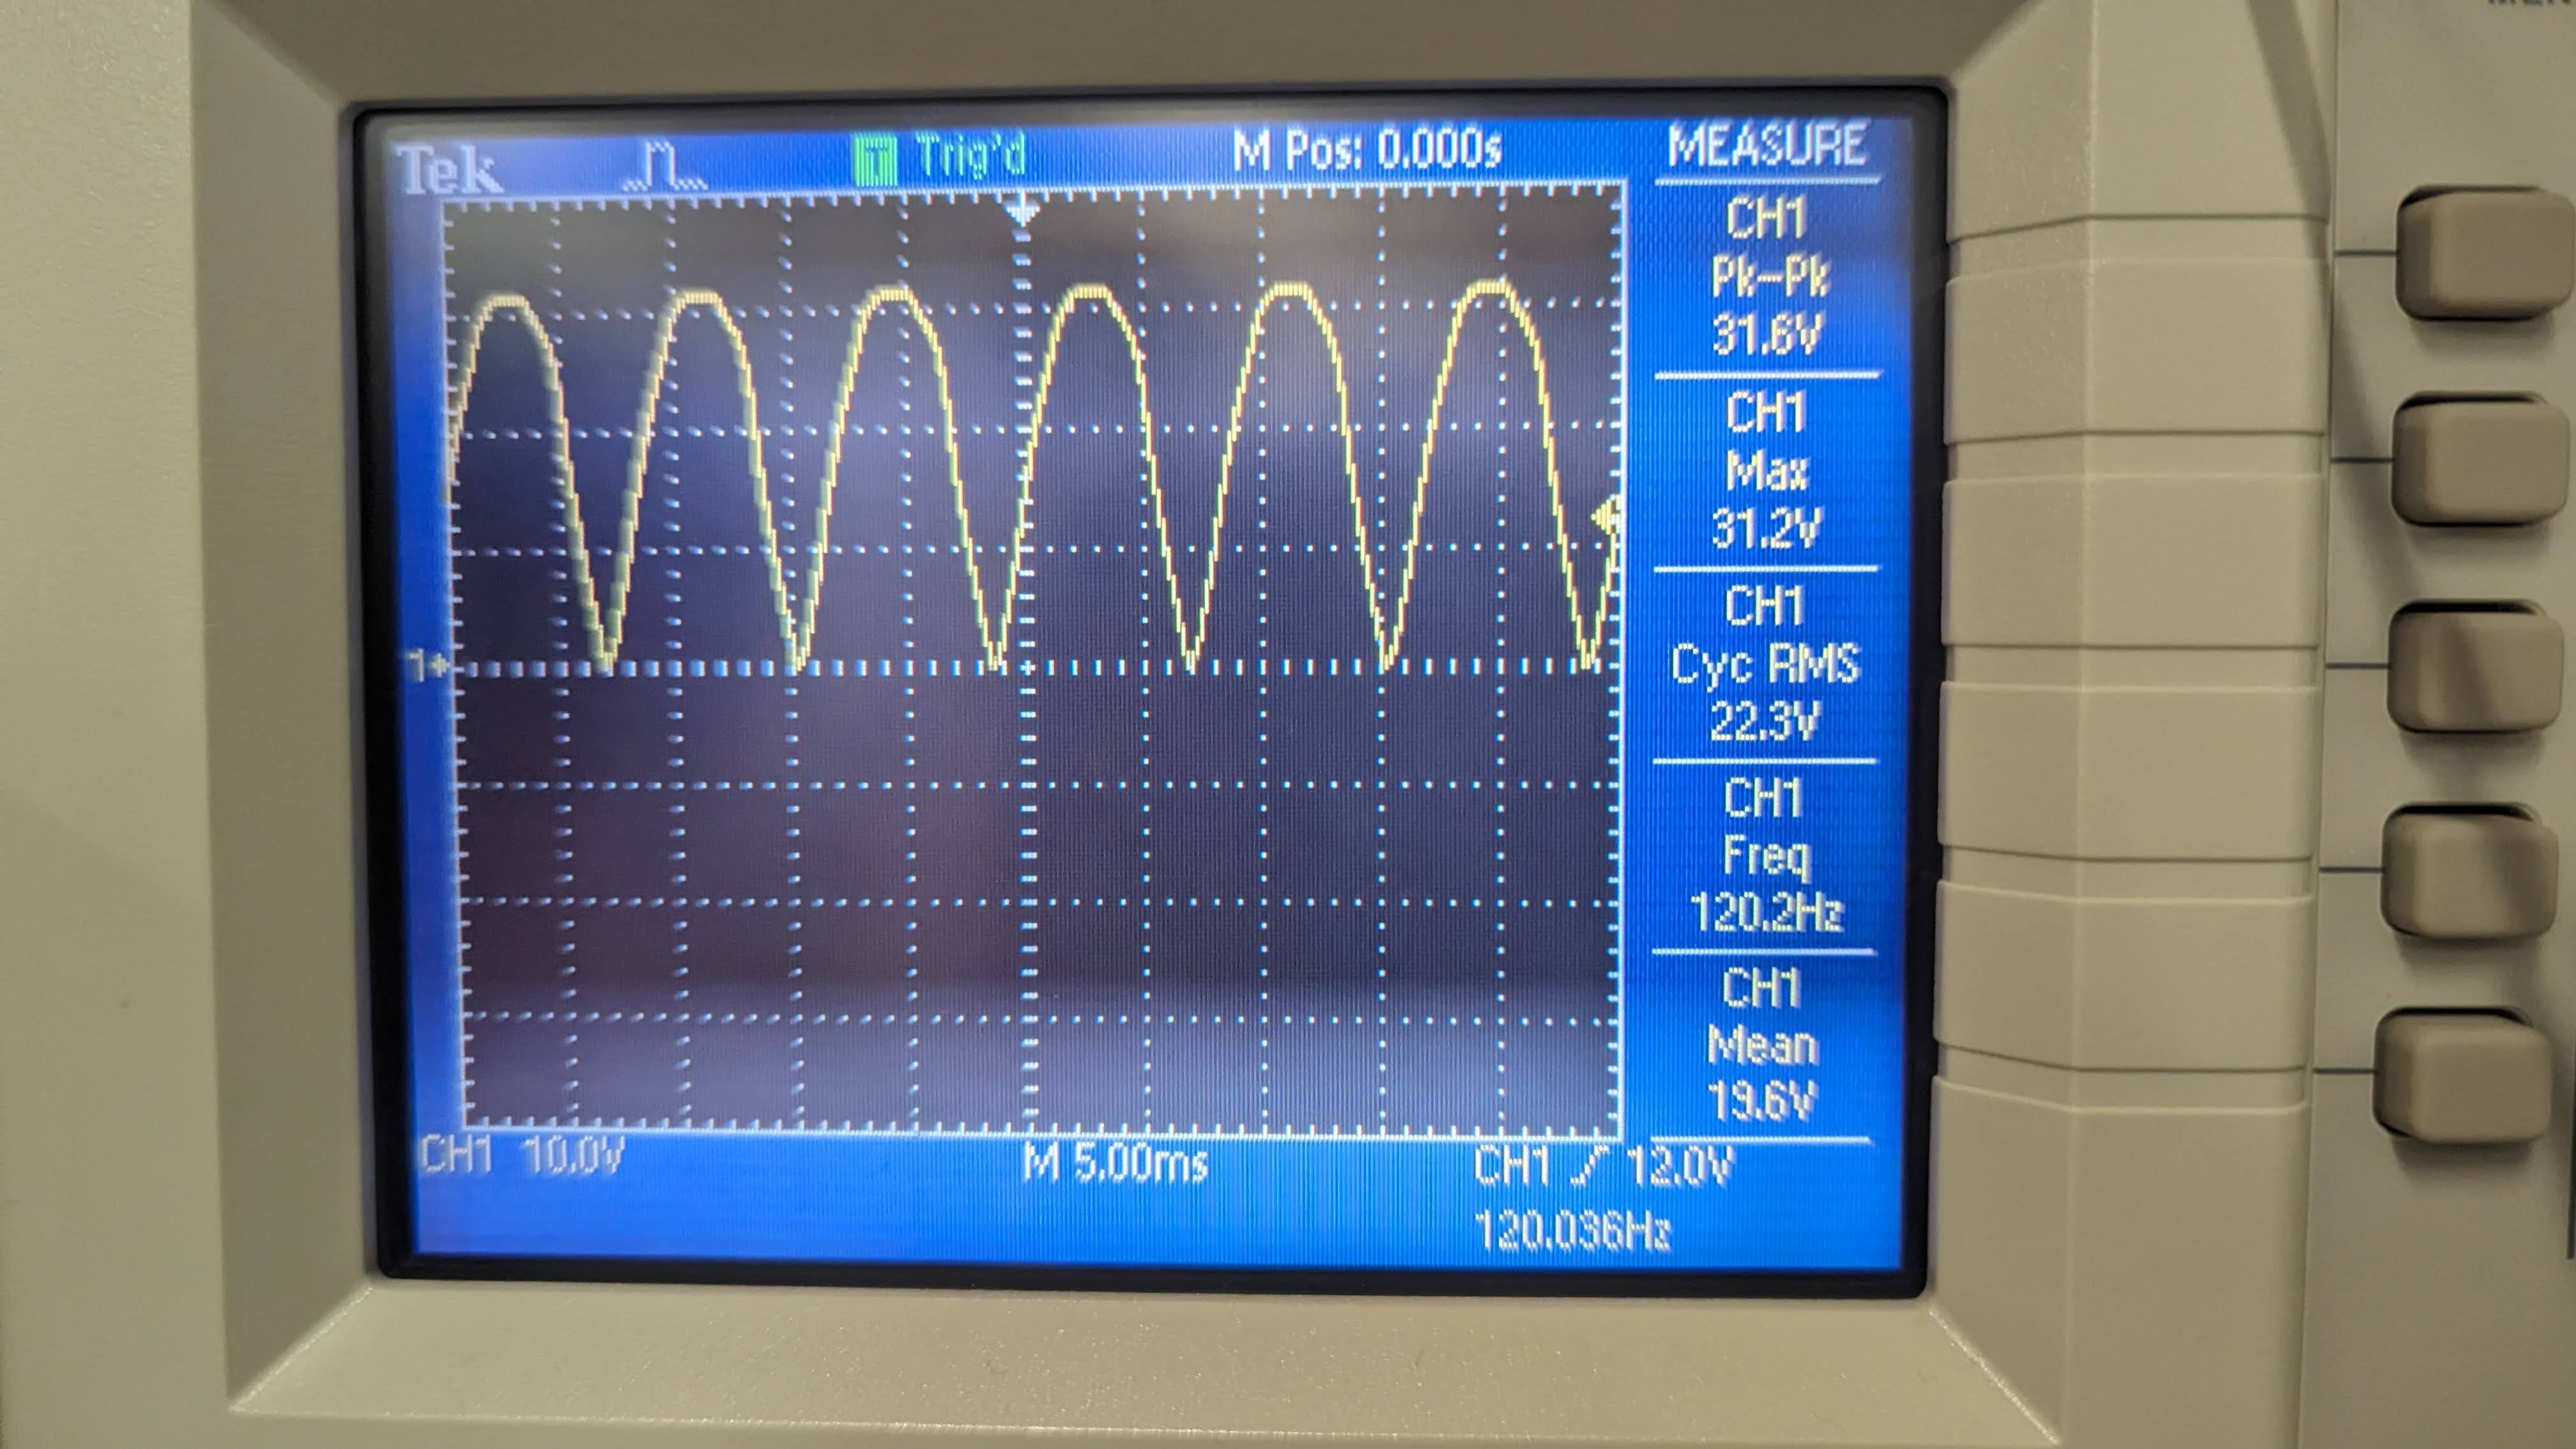
\includegraphics[width=0.45\textwidth]{lab1/t2p1a}
        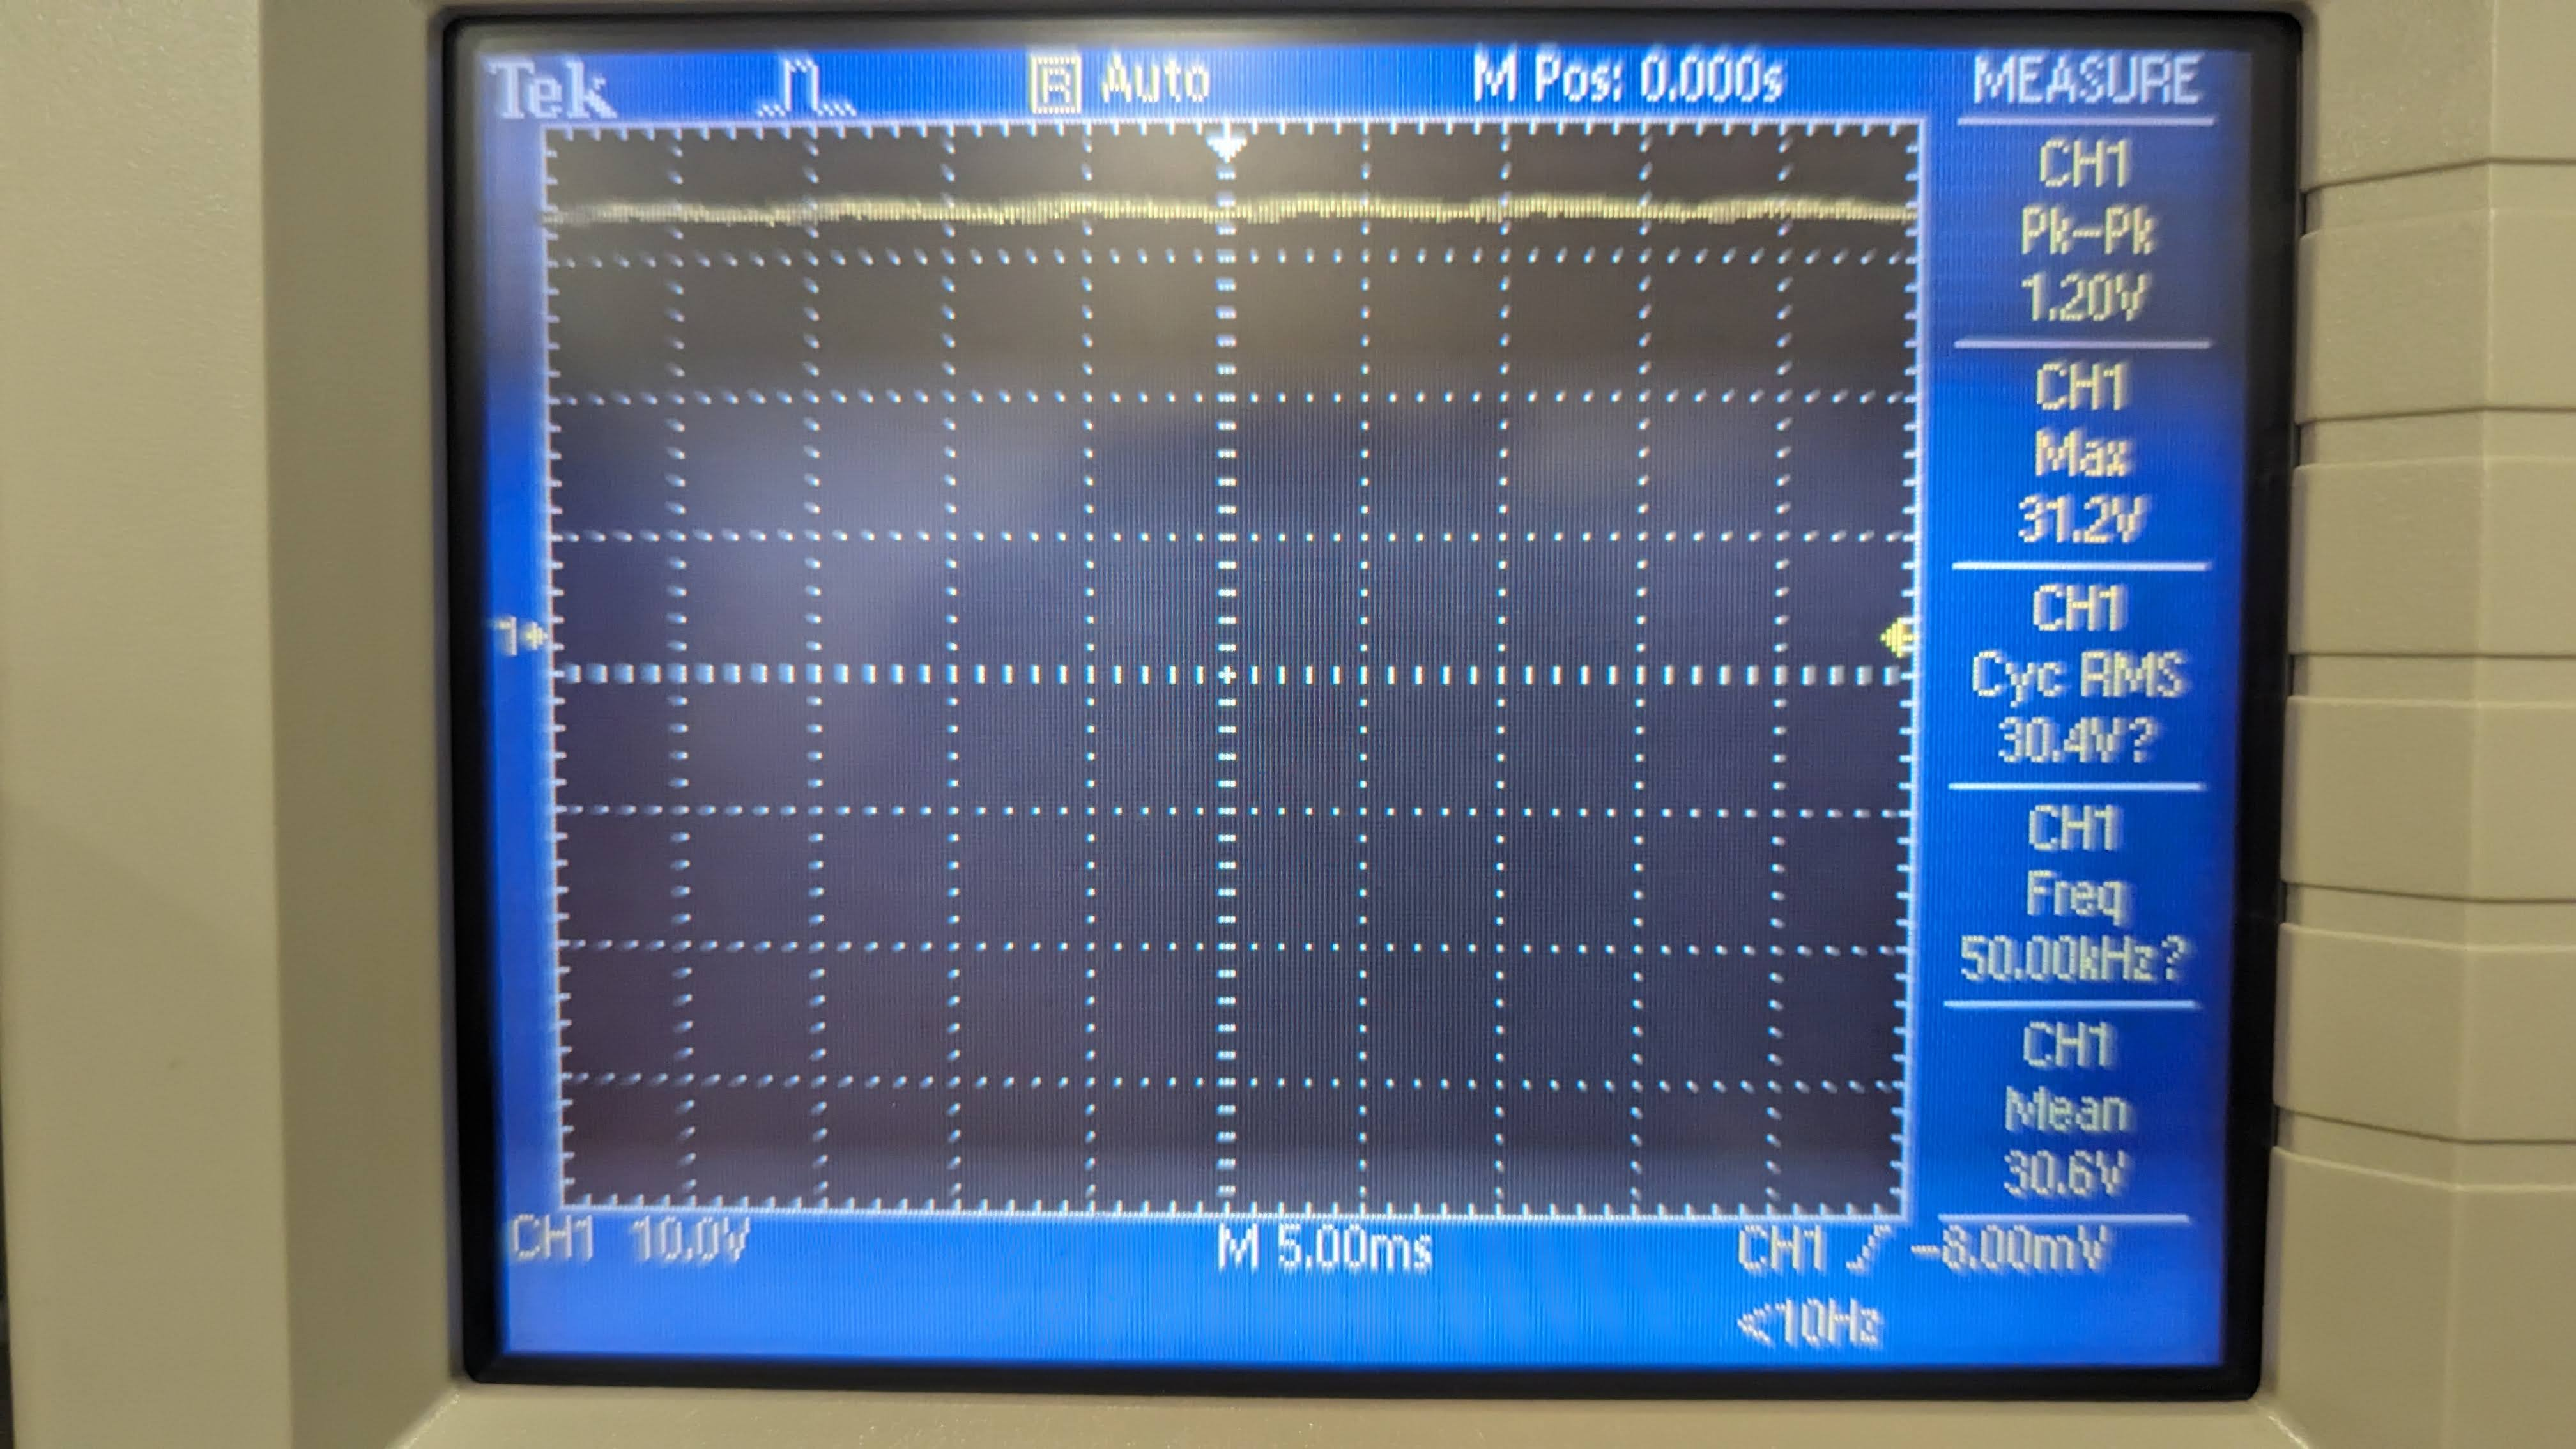
\includegraphics[width=0.45\textwidth]{lab1/t2p1b}
        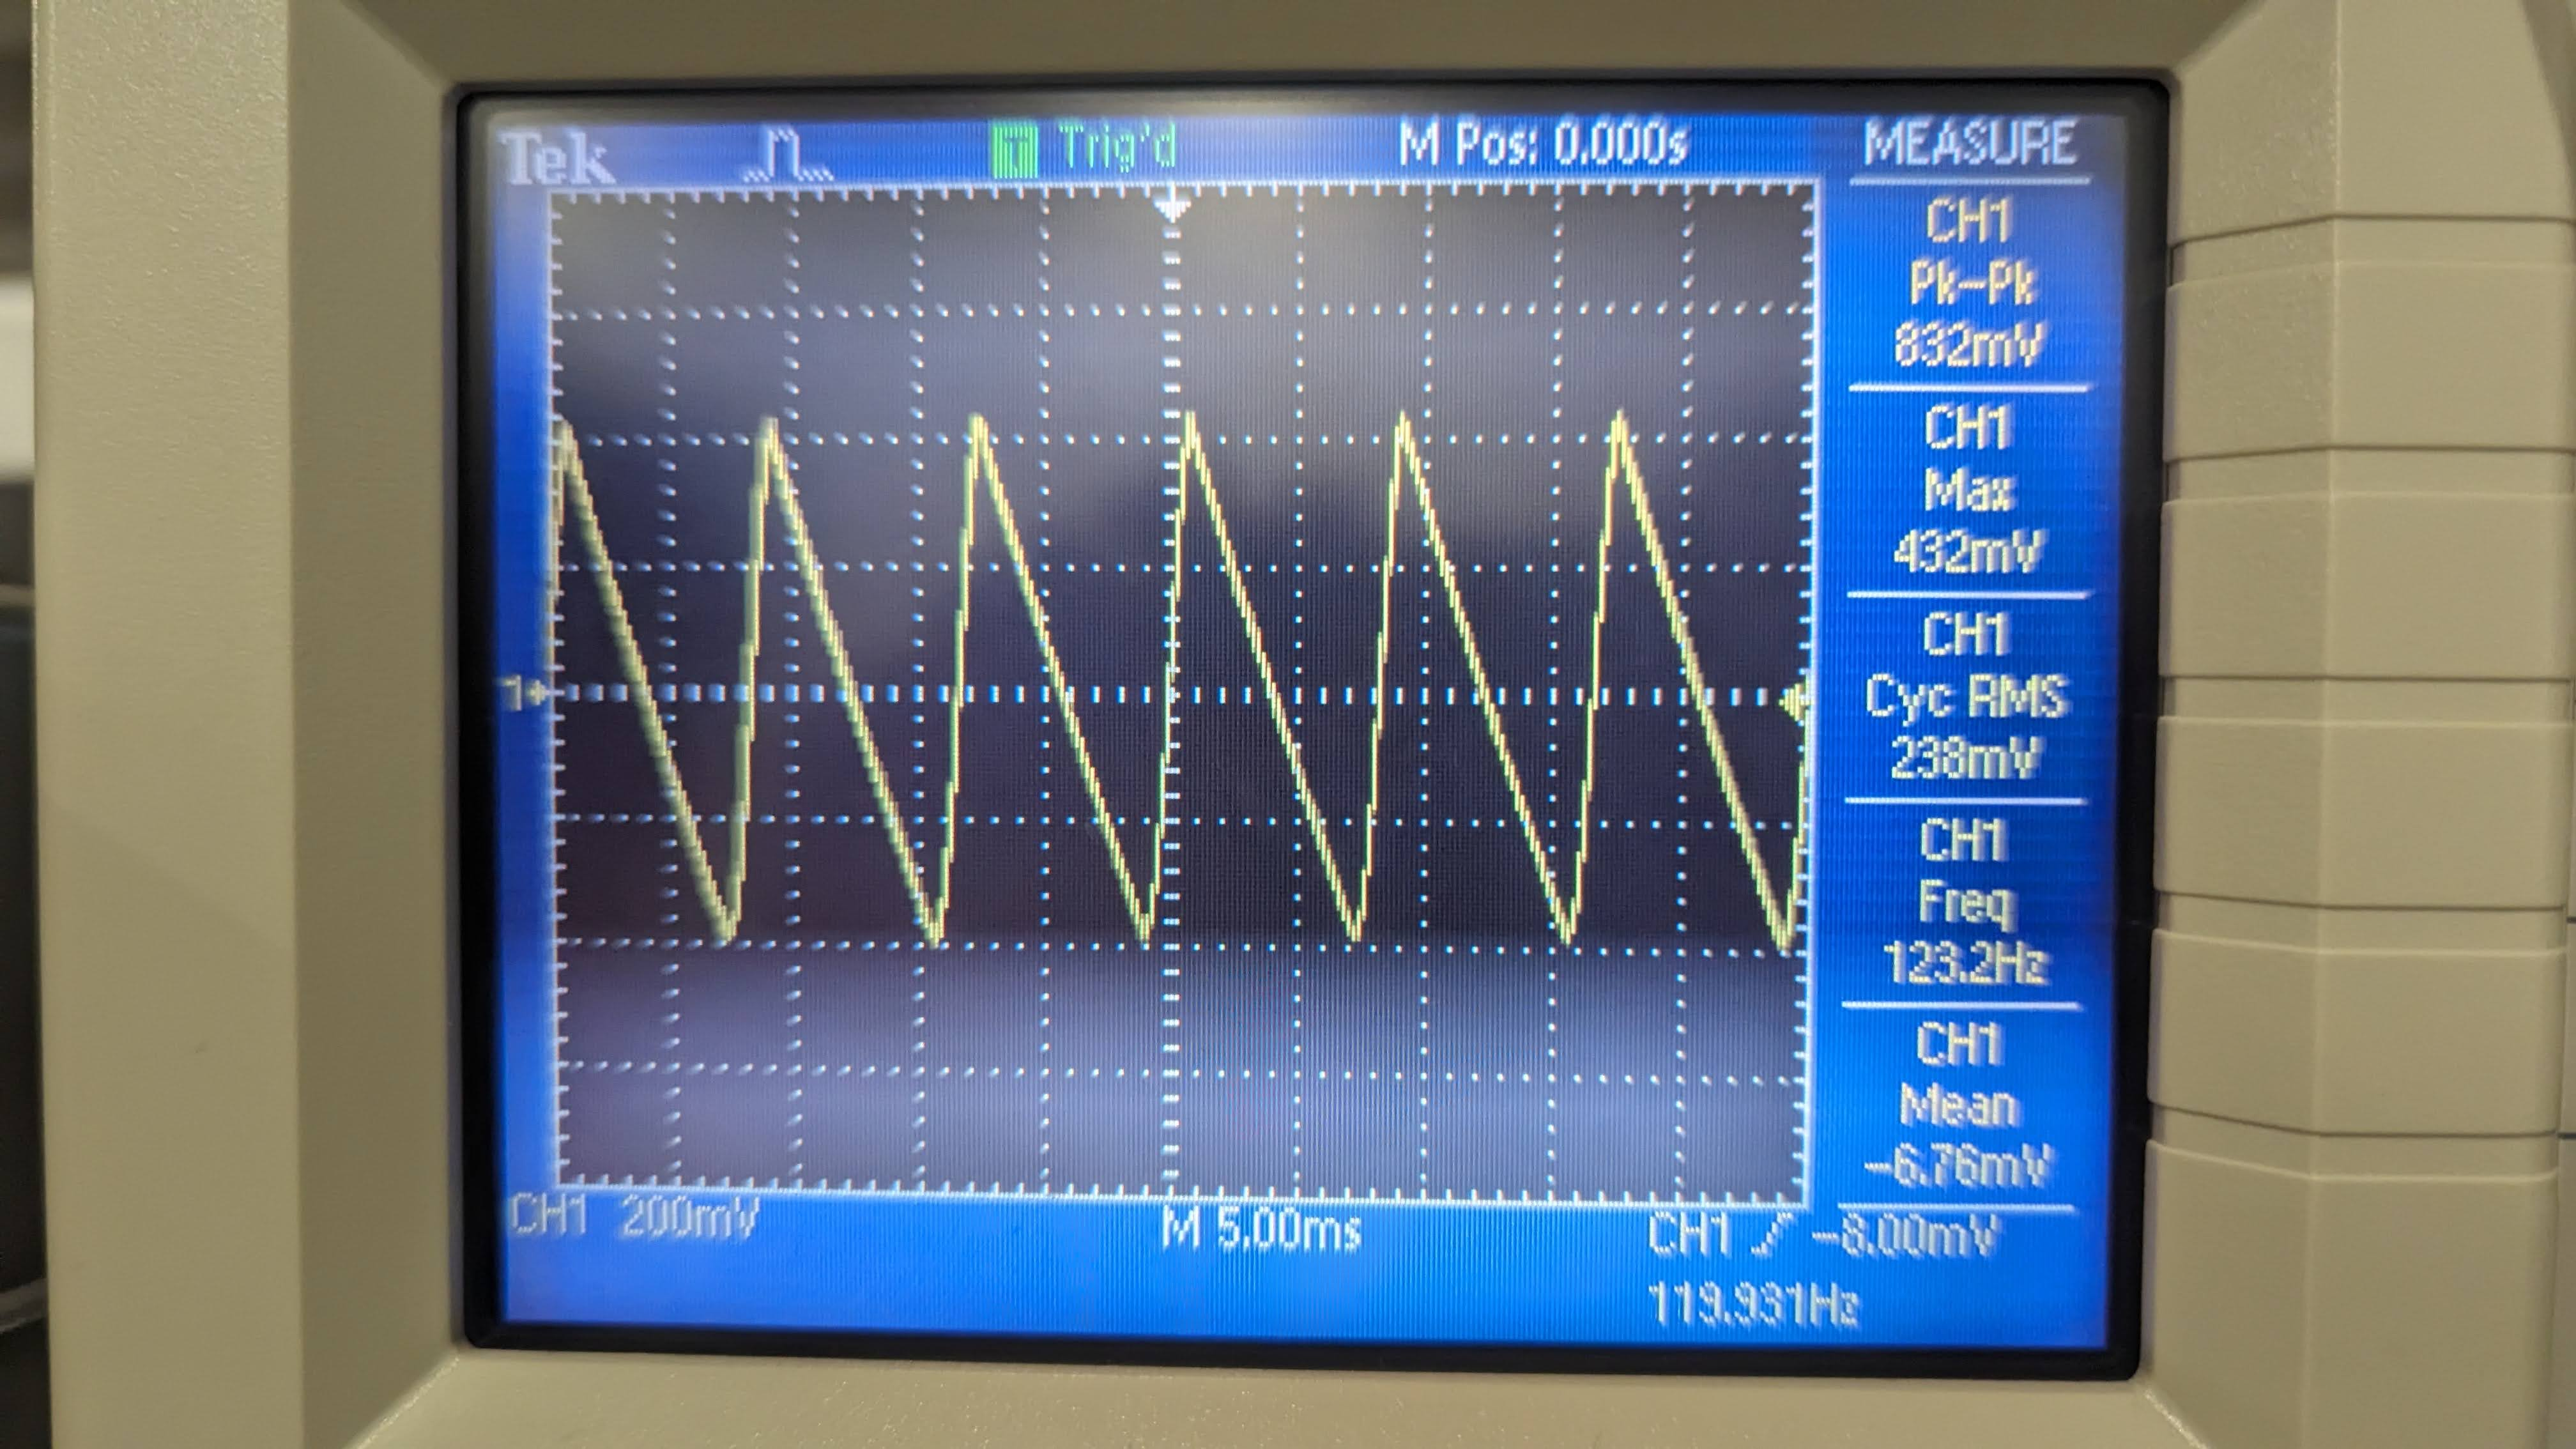
\includegraphics[width=0.45\textwidth]{lab1/t2p1c}
        \caption{Task 2, part 1 waveforms. Left top is $V_0$ with the capacitors, while the right top is $V_0$ without capacitors. Bottom is the AC-coupled ripple zoomed in, again the ripple (i.e. Pk-Pk) of $832$mV is less than $1$V.}
        \label{fig:t2p1}
\end{figure}

{\medskip\noindent\bf Part 2.} The procedure and setup was exactly the same as for part 1 of this task, see figure \ref{fig:t2b} for the setup.

\begin{figure}[htpb]
        \centering
        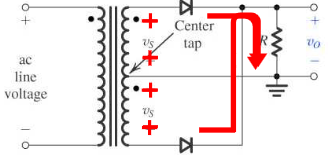
\includegraphics[width=0.5\textwidth]{t2b}
        \caption{Setup for part 2 of task 2. This diagram was taken from the lecture slides.}
        \label{fig:t2b}
\end{figure}

Again, the capacitor comes from the equation:
\[
C = \frac{V_p-V_d}{2fR_LV_r}=\frac{16.8-0.7}{2\cdot 60\cdot 1000\cdot 1}=134\mu\text{F}
.\]
Three 33$\mu$F capacitors were used in parallel to simulate this. The waveforms are in figure \ref{fig:t2p2}. The peak voltage before the capacitors was 16.4V. After adding them, the average voltage of the smoothed wave was $15.9$V. This is consistent with the expectation that the average voltage should be $V_p- \frac{V_r}{2}=16.4-0.5=15.9$V. Finally the ripple was $944$mV.

In terms of comparison, this setup is very similar to task 1 with the half wave rectifier, with the only difference being that, as the name implies, it rectifies the entire wave rather than every second peak.

\begin{figure}[htpb]
        \centering
        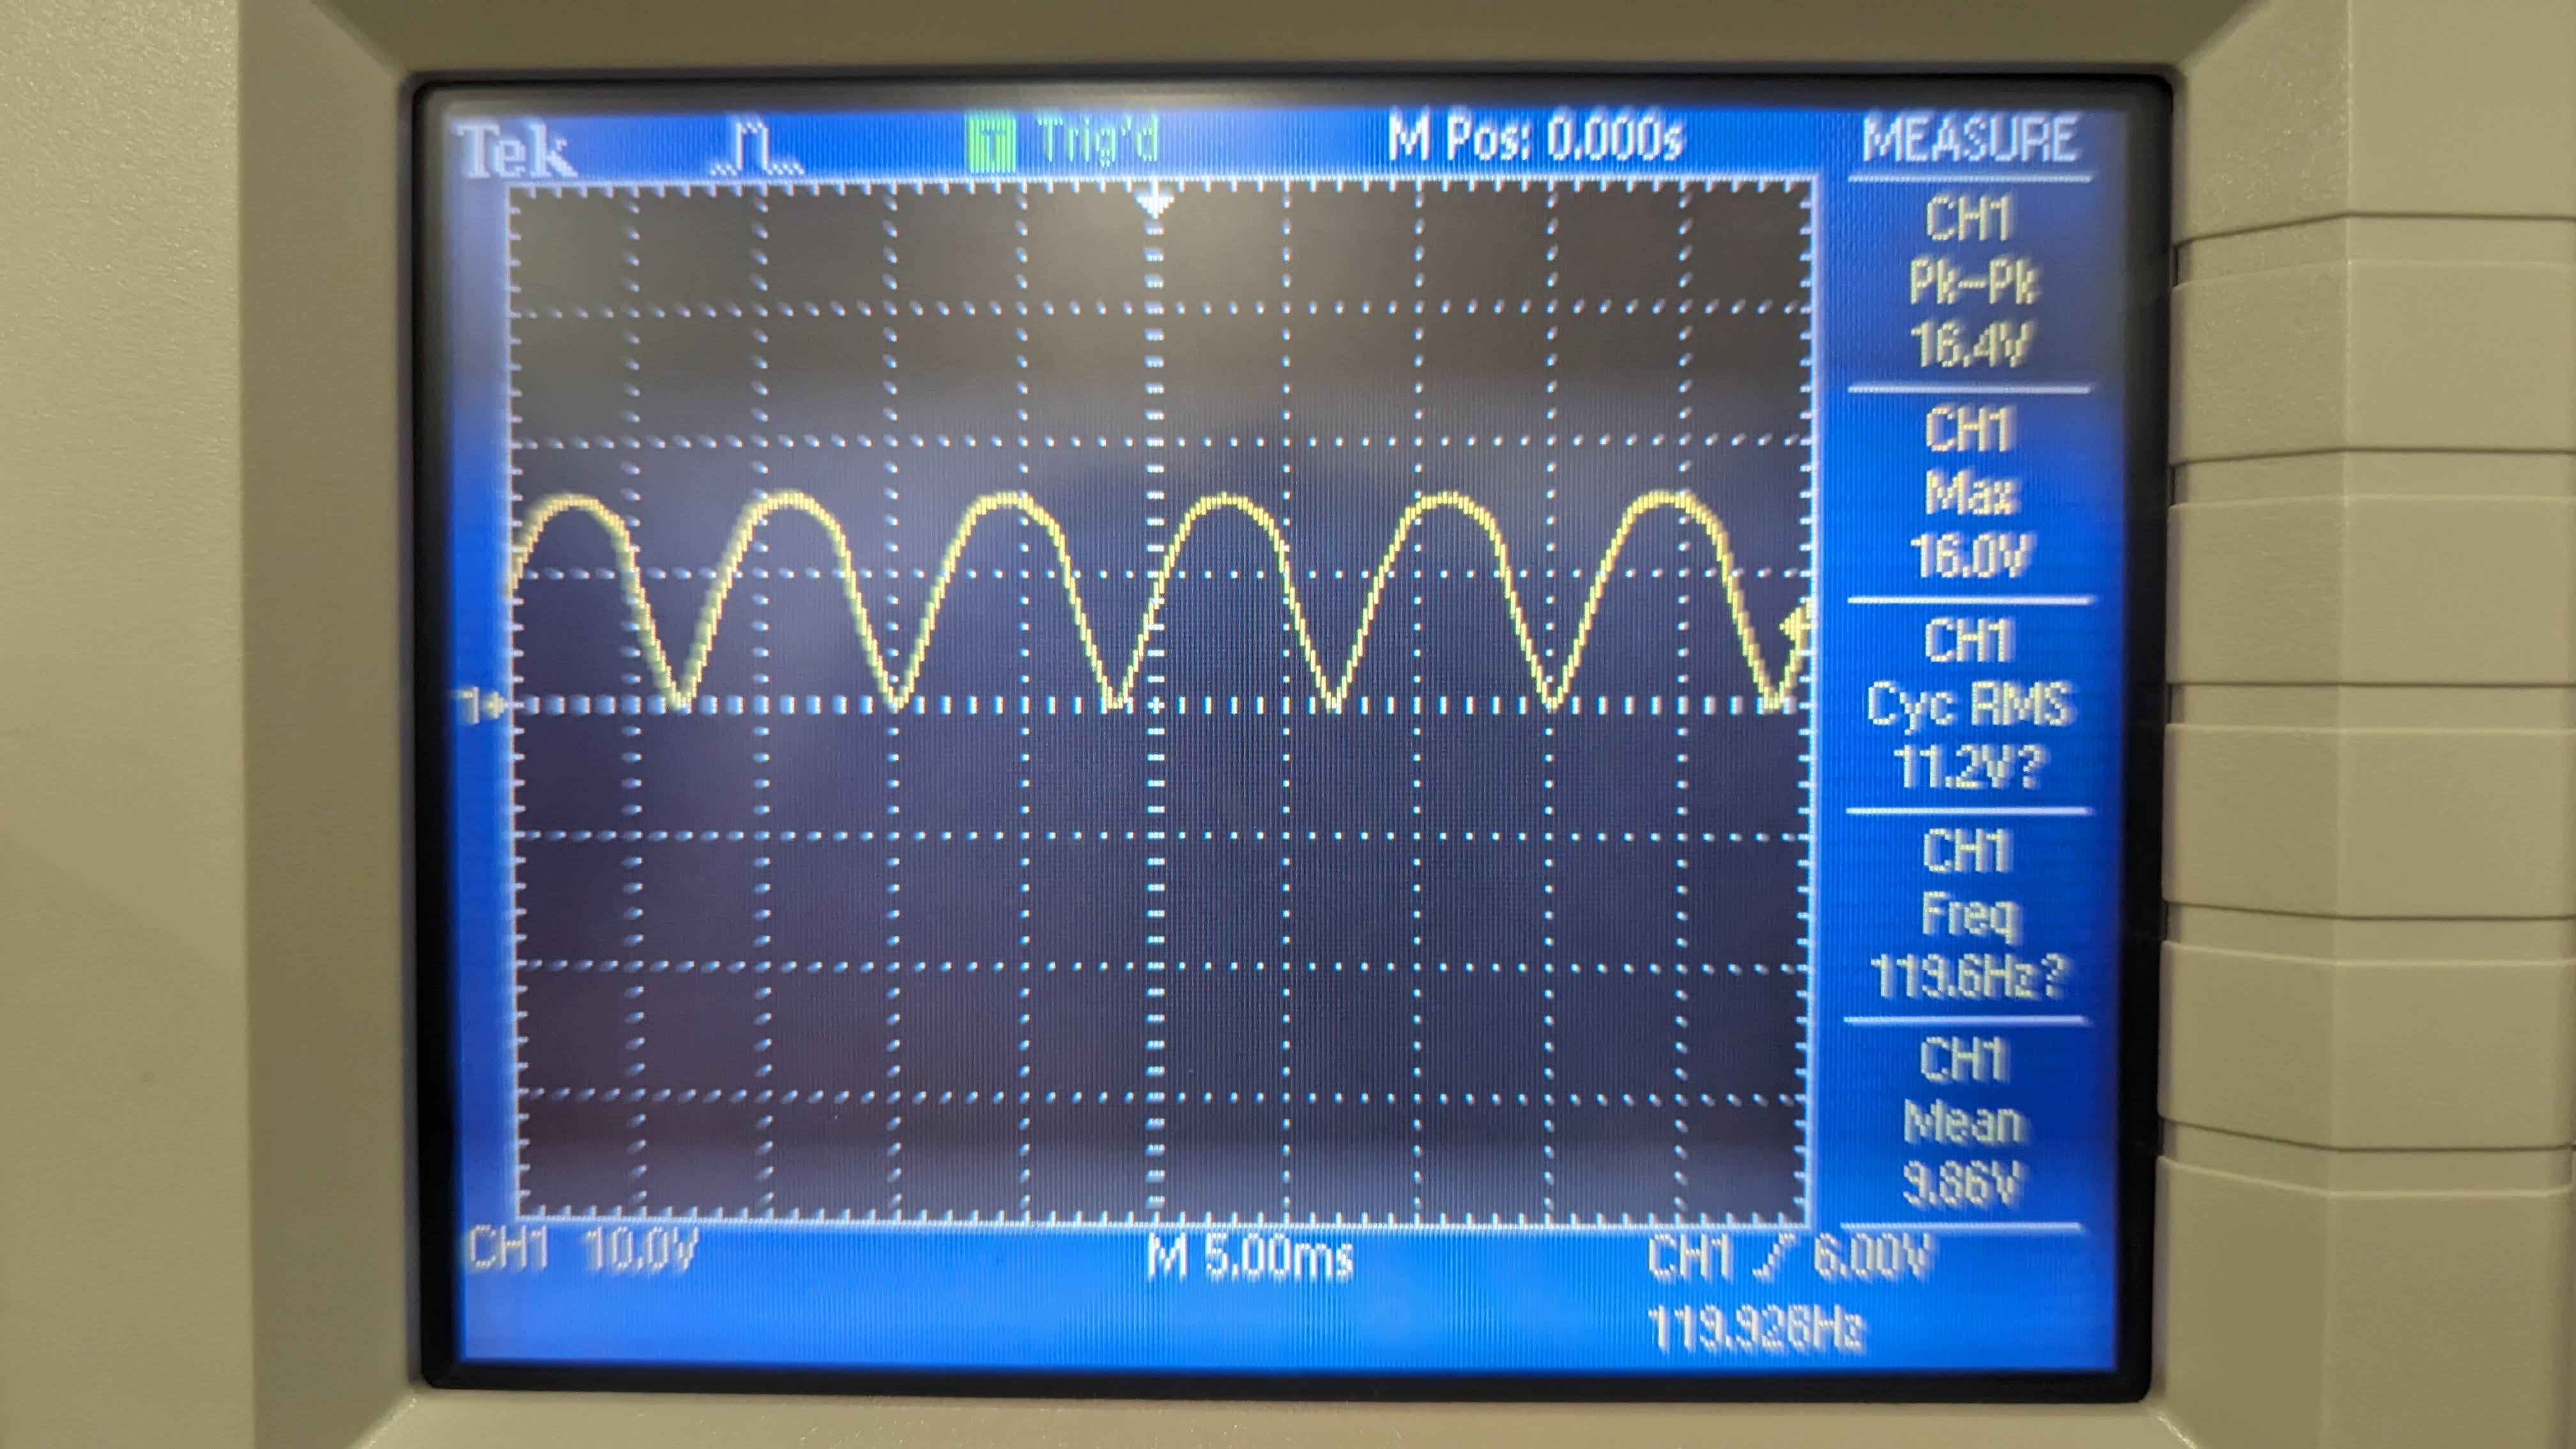
\includegraphics[width=0.45\textwidth]{lab1/t2p2a}
        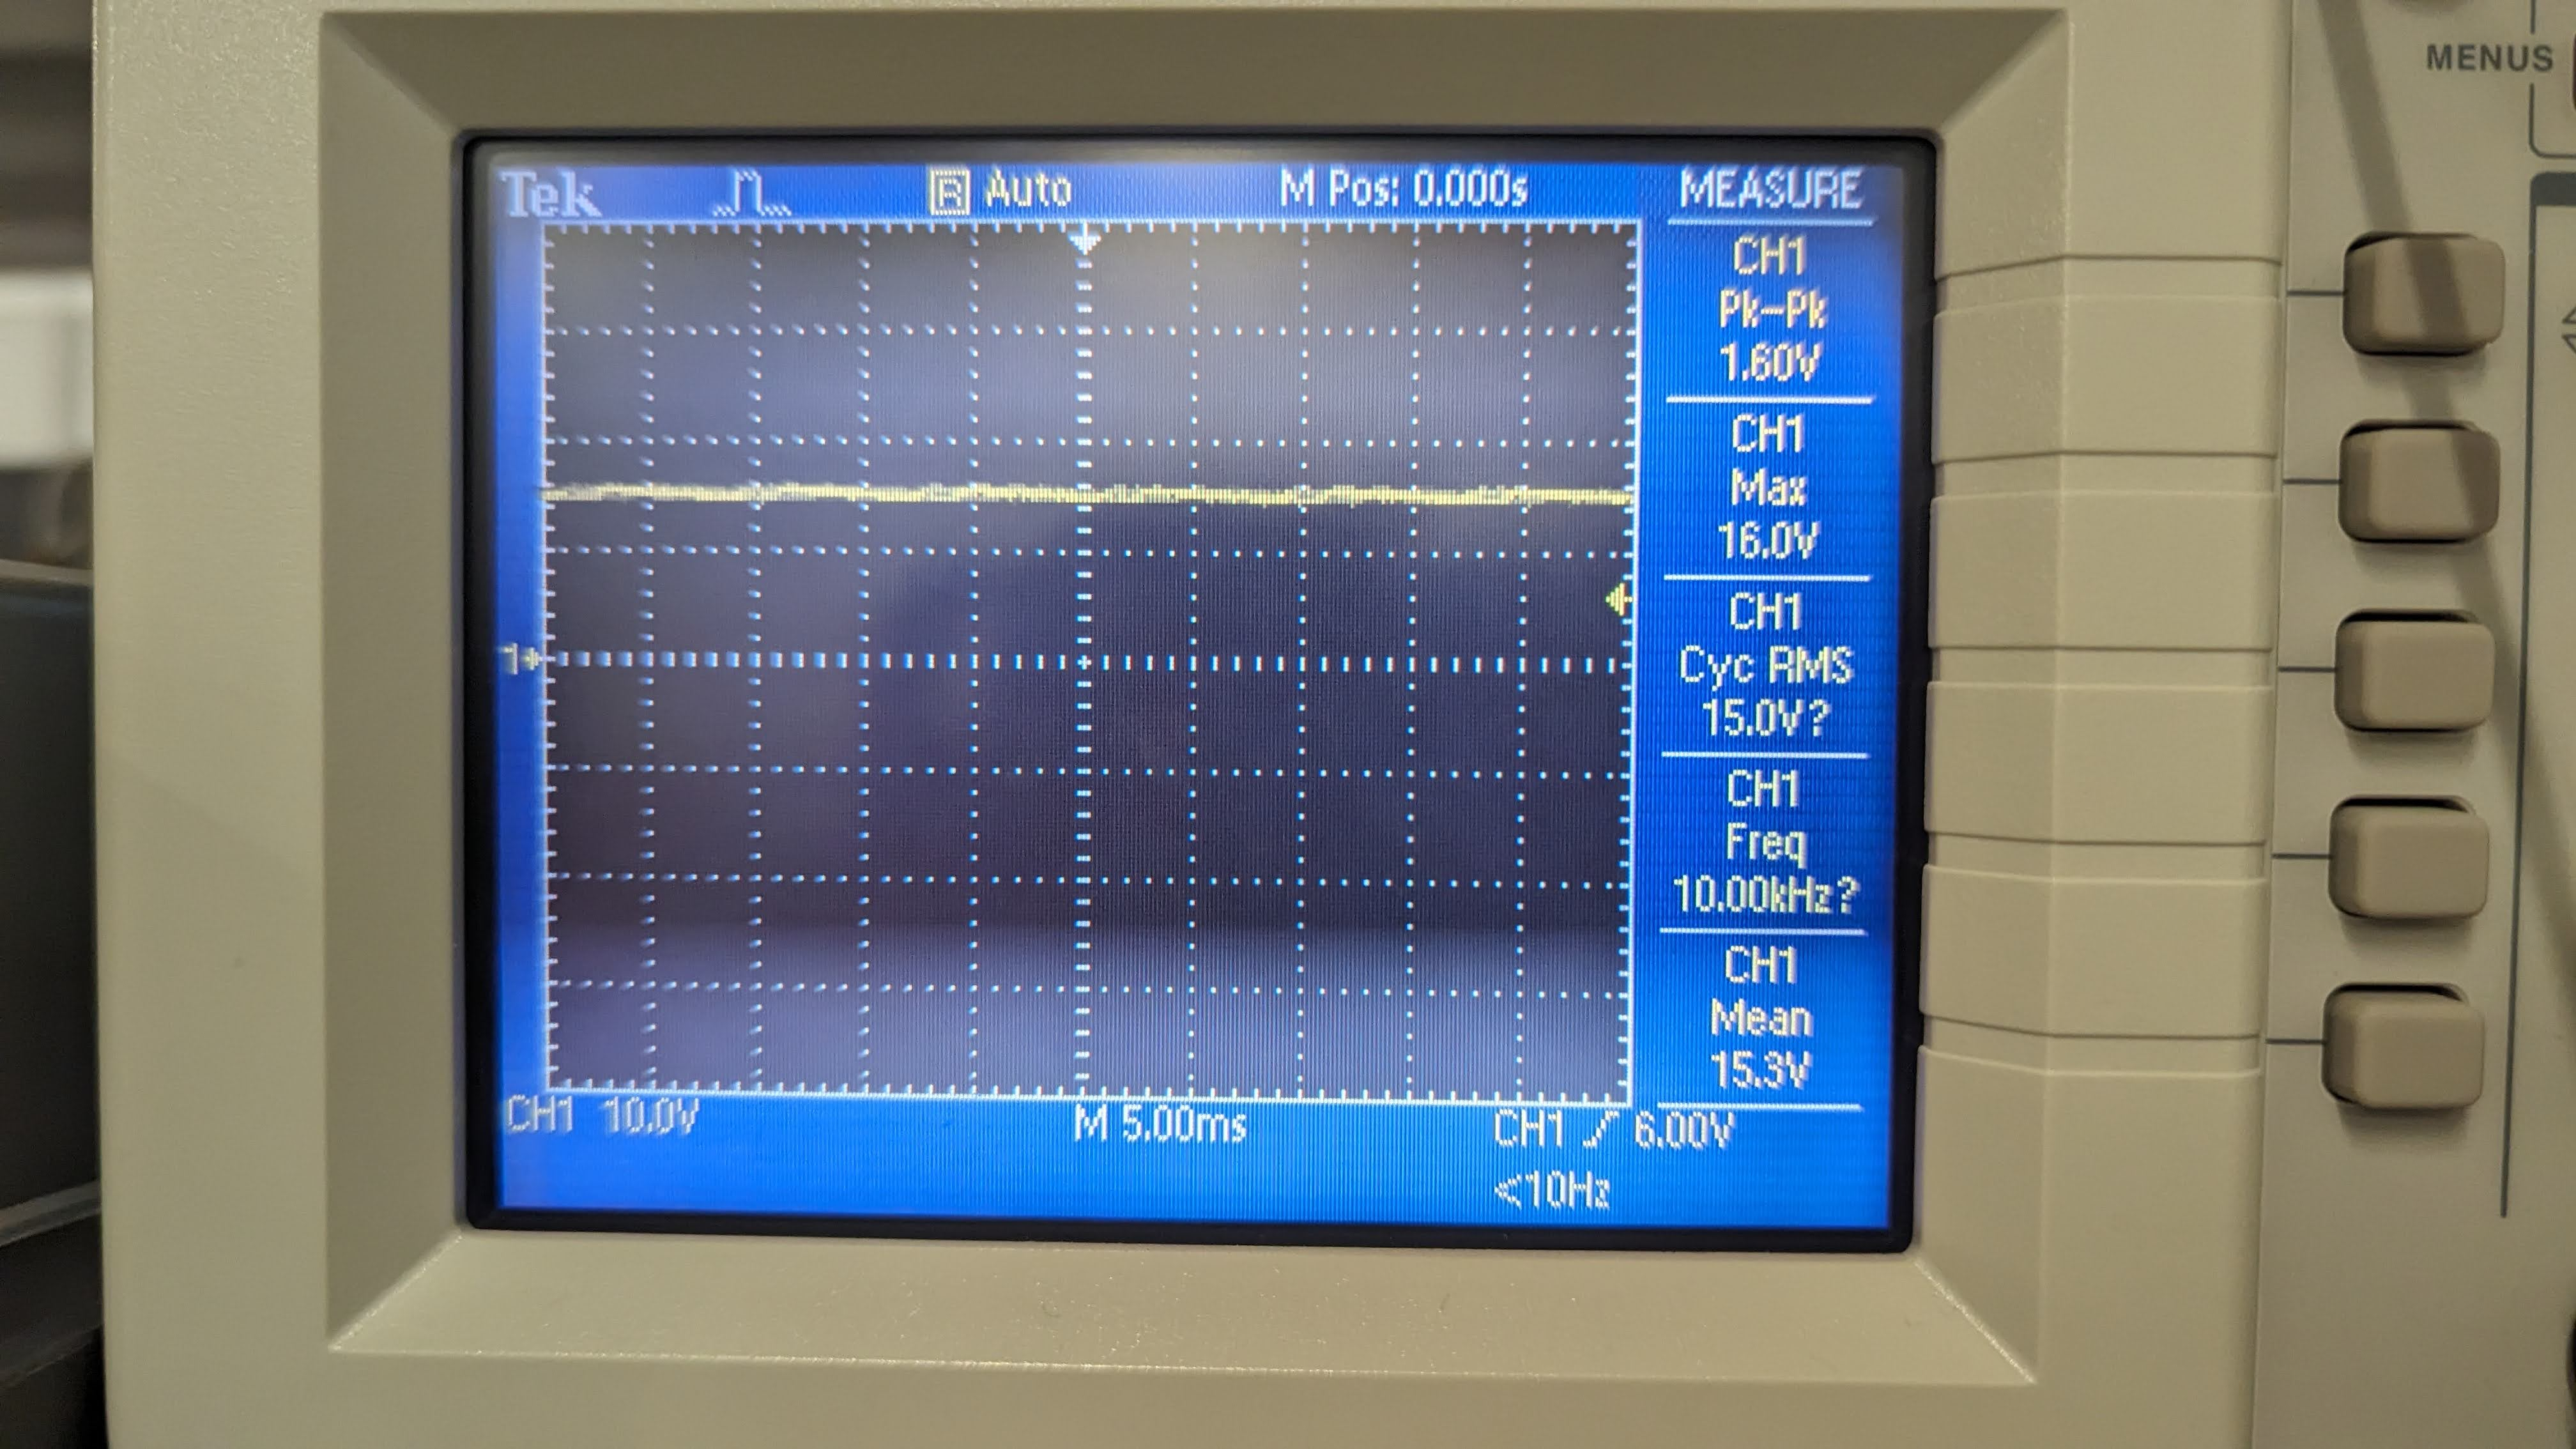
\includegraphics[width=0.45\textwidth]{lab1/t2p2b}
        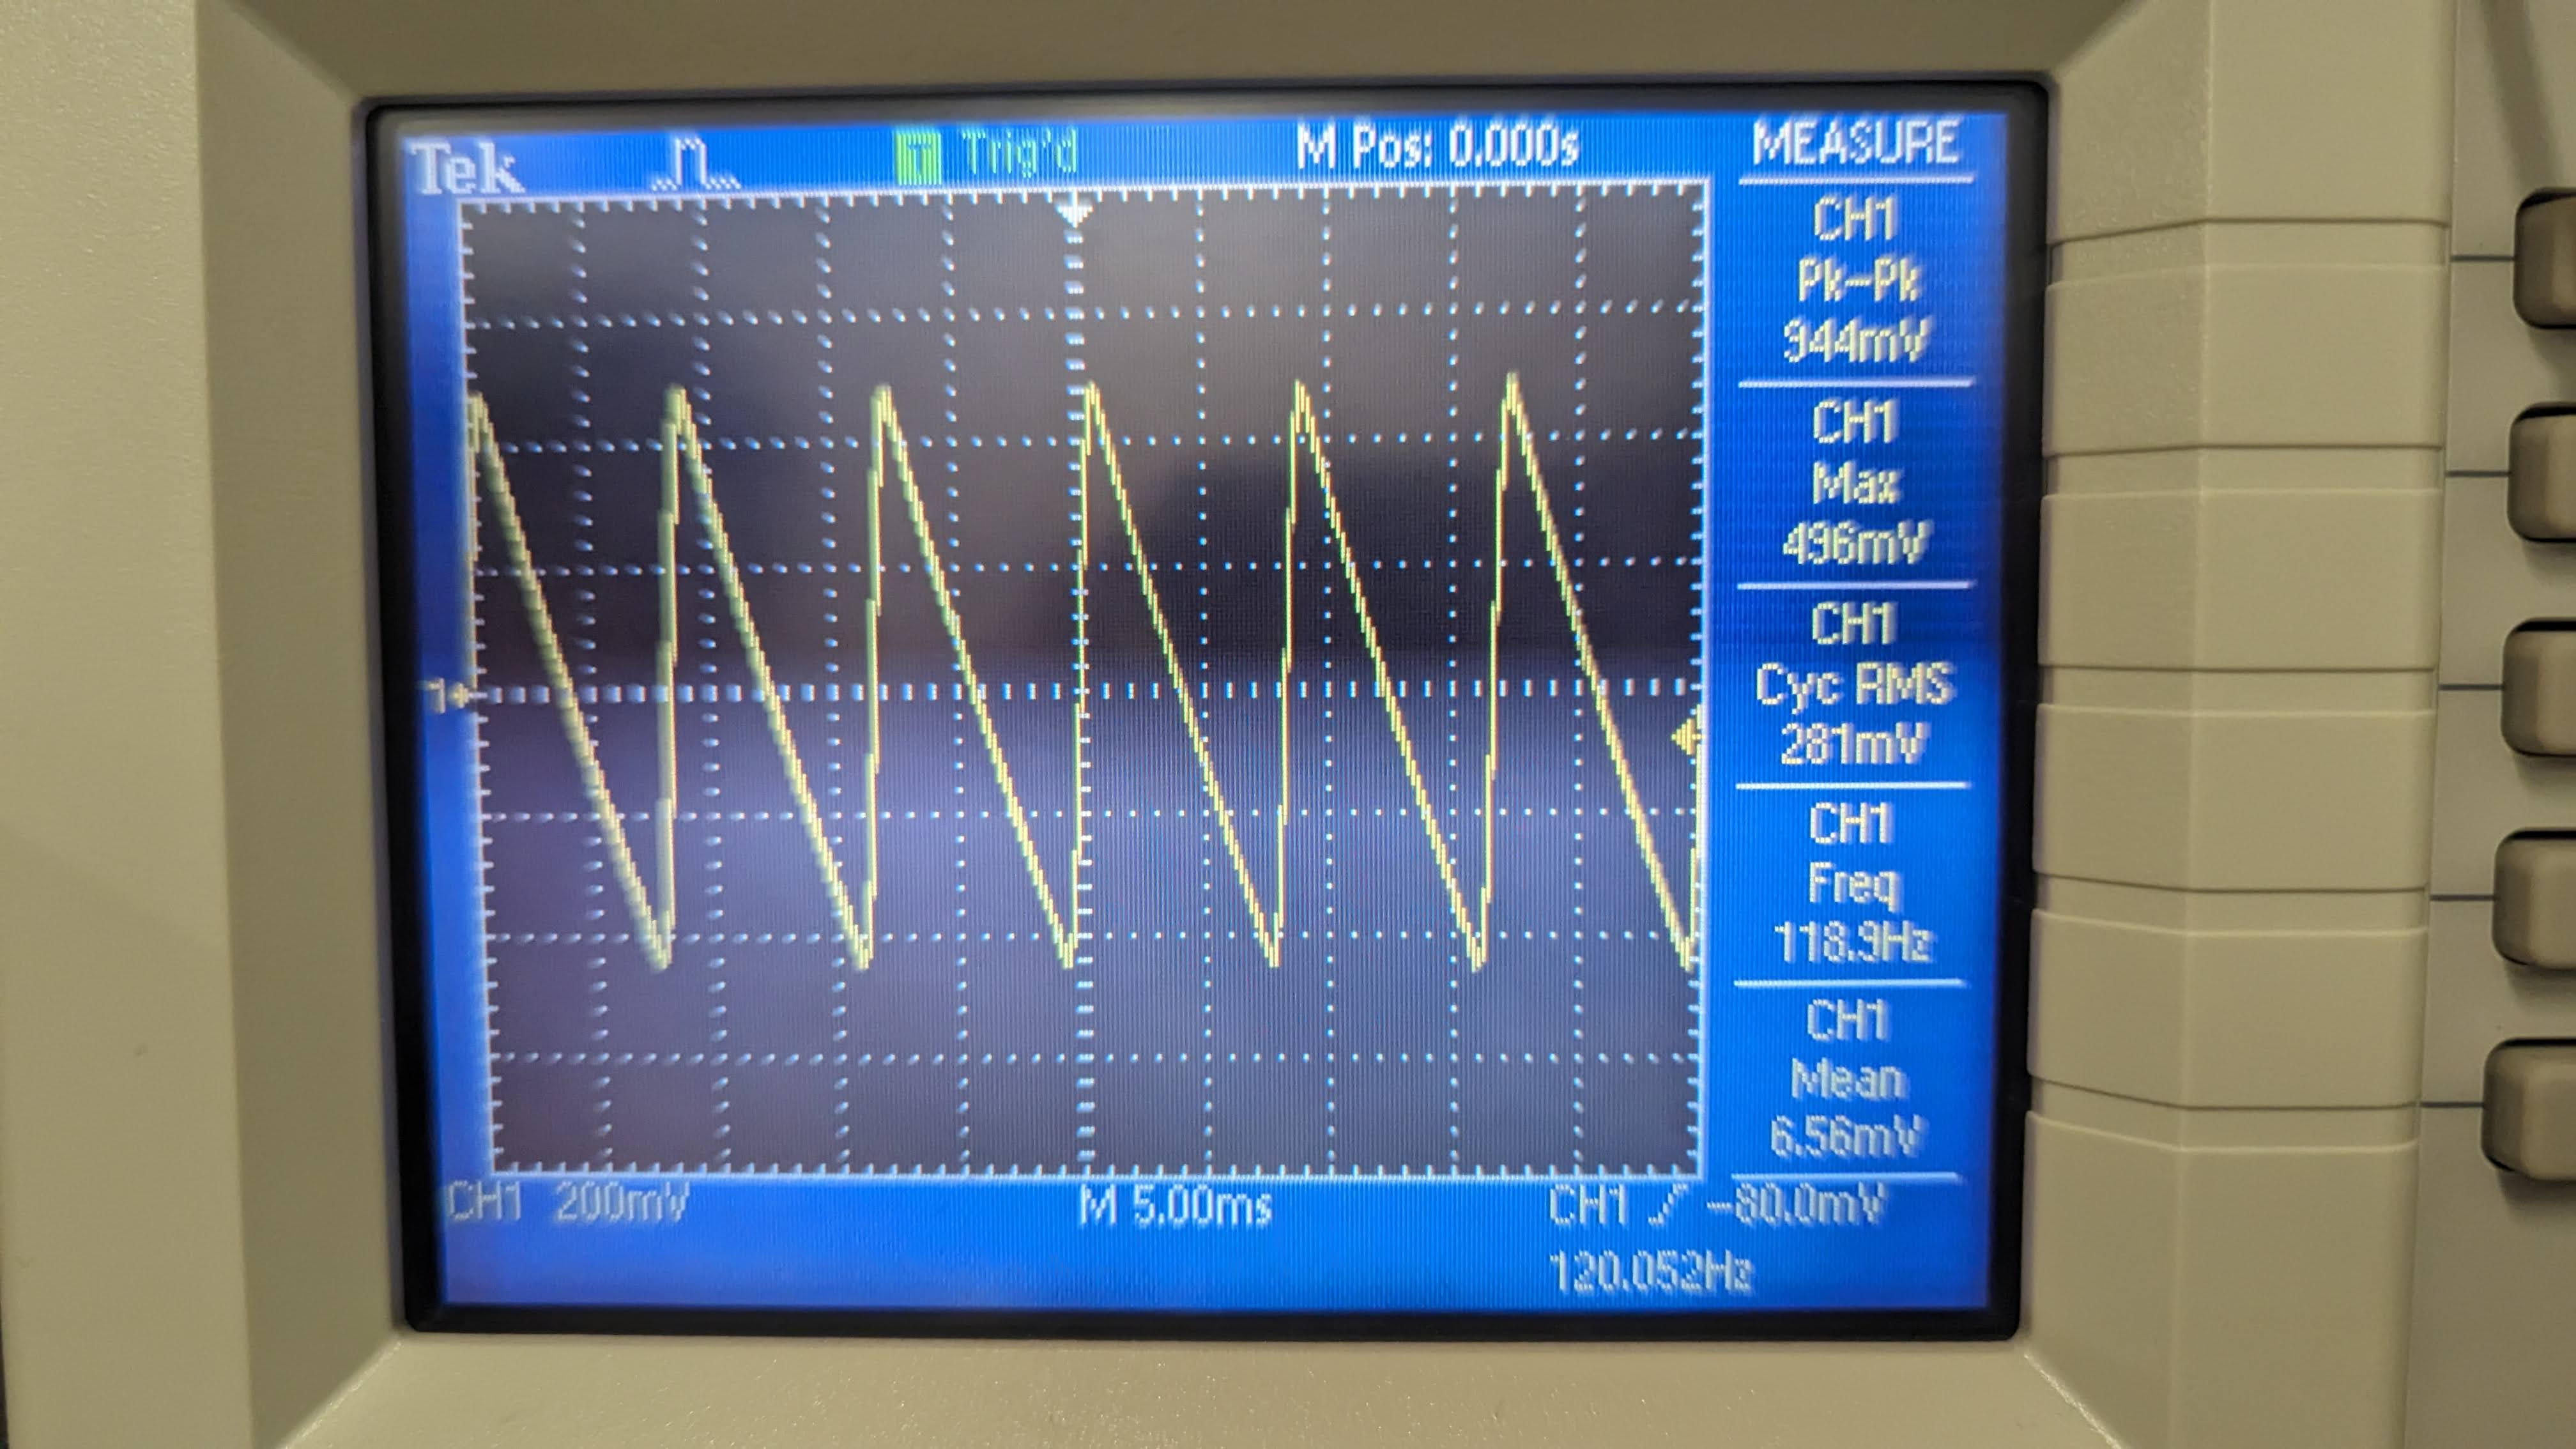
\includegraphics[width=0.45\textwidth]{lab1/t2p2c}
        \caption{Task 2, part 2 waveforms. Left top is $V_0$ with the capacitors, while the right top is $V_0$ without capacitors. Bottom is the AC-coupled ripple zoomed in, again the ripple (i.e. Pk-Pk) of $944$mV is less than $1$V.}
        \label{fig:t2p2}
\end{figure}

{\medskip\noindent\bf Question 3.} The diagram of the setup can be seen in figure \ref{fig:t3}. After setting up this circuit, we first measured the DC voltage by getting the outputted waveform. This was found to be 4.81. Next we found the output ripple voltage by using AC coupling, which was found to be 118mV. The waveforms used can be seen in figure \ref{fig:t3w}

Obviously the ripple is an order of magnitude smaller than what was seen in tasks 1 or 2, which is a major difference. However, doing the math using the formula found in the lecture 4 slides page 5, one would actually expect a much smaller ripple:
\[
        \frac{\Delta V_0}{\Delta V_{in}}\bigg|_{I=\text{constant}}= \frac{r_Z}{R_L+r_z}= \frac{1.5}{1000+1.5}=1.47\text{mV/V}
.\]
There are a few possible reasons for the discrepancy. It could be a faulty Zender diode, although I consider this fairly unlikely. We also could have measured the wrong line for this measurement, but there are only a few possible voltages to measure in a circuit this simple and none of them have a value close to $100$mV. Another possibility is that either a resistor or capacitor was mixed up and mistakenly used despite us attempting to double check using the DMM beforehand, which would definitely affect the reading. Finally, the datasheet for the zener diode isn't entirely clear on what exactly its zener resistance is, so there's a possibility that it was misinterpreted here which would make the above calculation irrelevant. Regardless of the exact reason, the difference wasn't noticed until after the conclusion of the lab so a remeasurement wasn't possible.

This task showcases the zener diodes capabilities as a fantastic filter for a voltage regulator. By adding it, we reduced the ripple voltage by an order of magnitude. This is very useful for DC applications where a smooth voltage is required.

\begin{figure}[htpb]
        \centering
        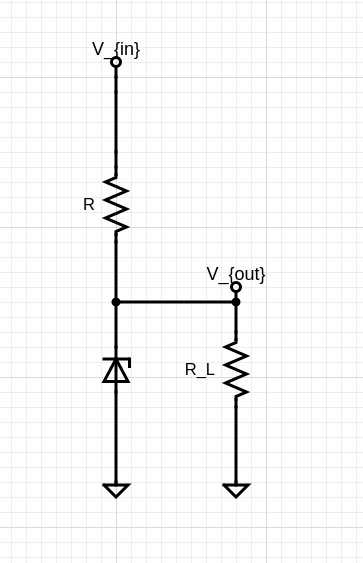
\includegraphics[width=0.3\textwidth]{q4}
        \caption{Circuit diagram for part 3 (same as prelab), with $V_{in}$ being attached to $V_0$ in figure \ref{fig:t2p2}.}
        \label{fig:t3}
\end{figure}

\begin{figure}[htpb]
        \centering
        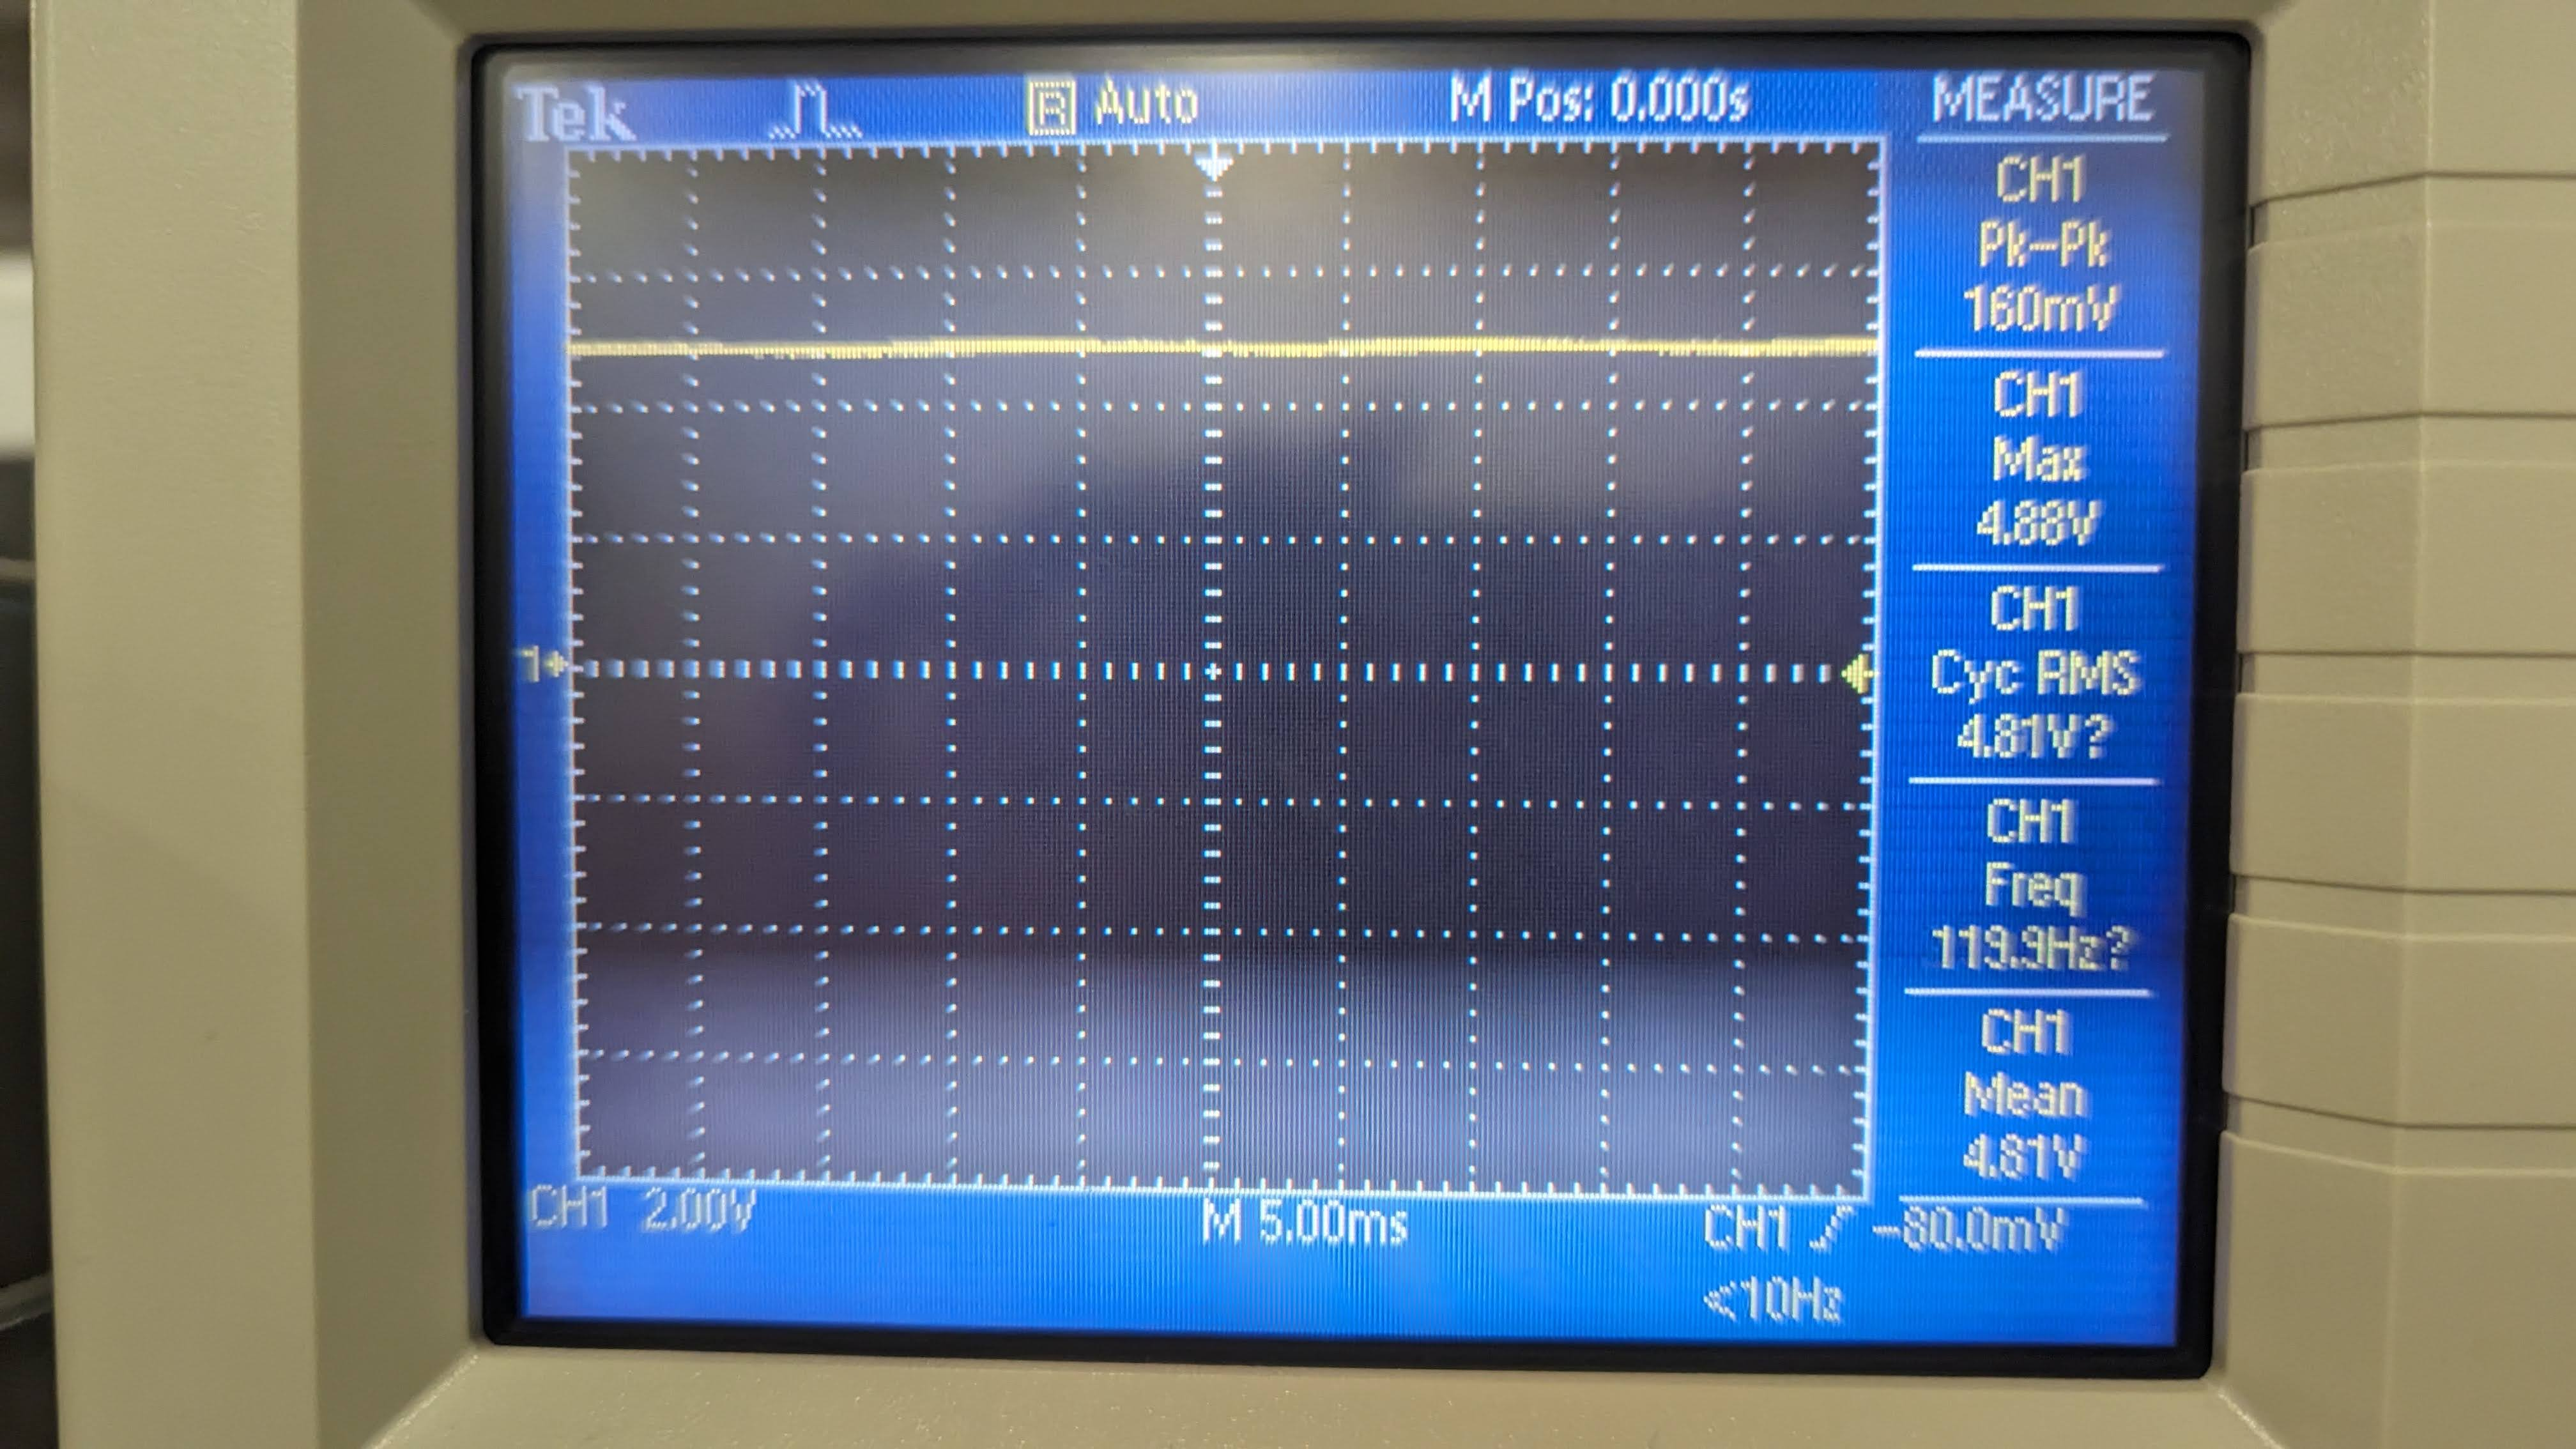
\includegraphics[width=0.45\textwidth]{lab1/t3a}
        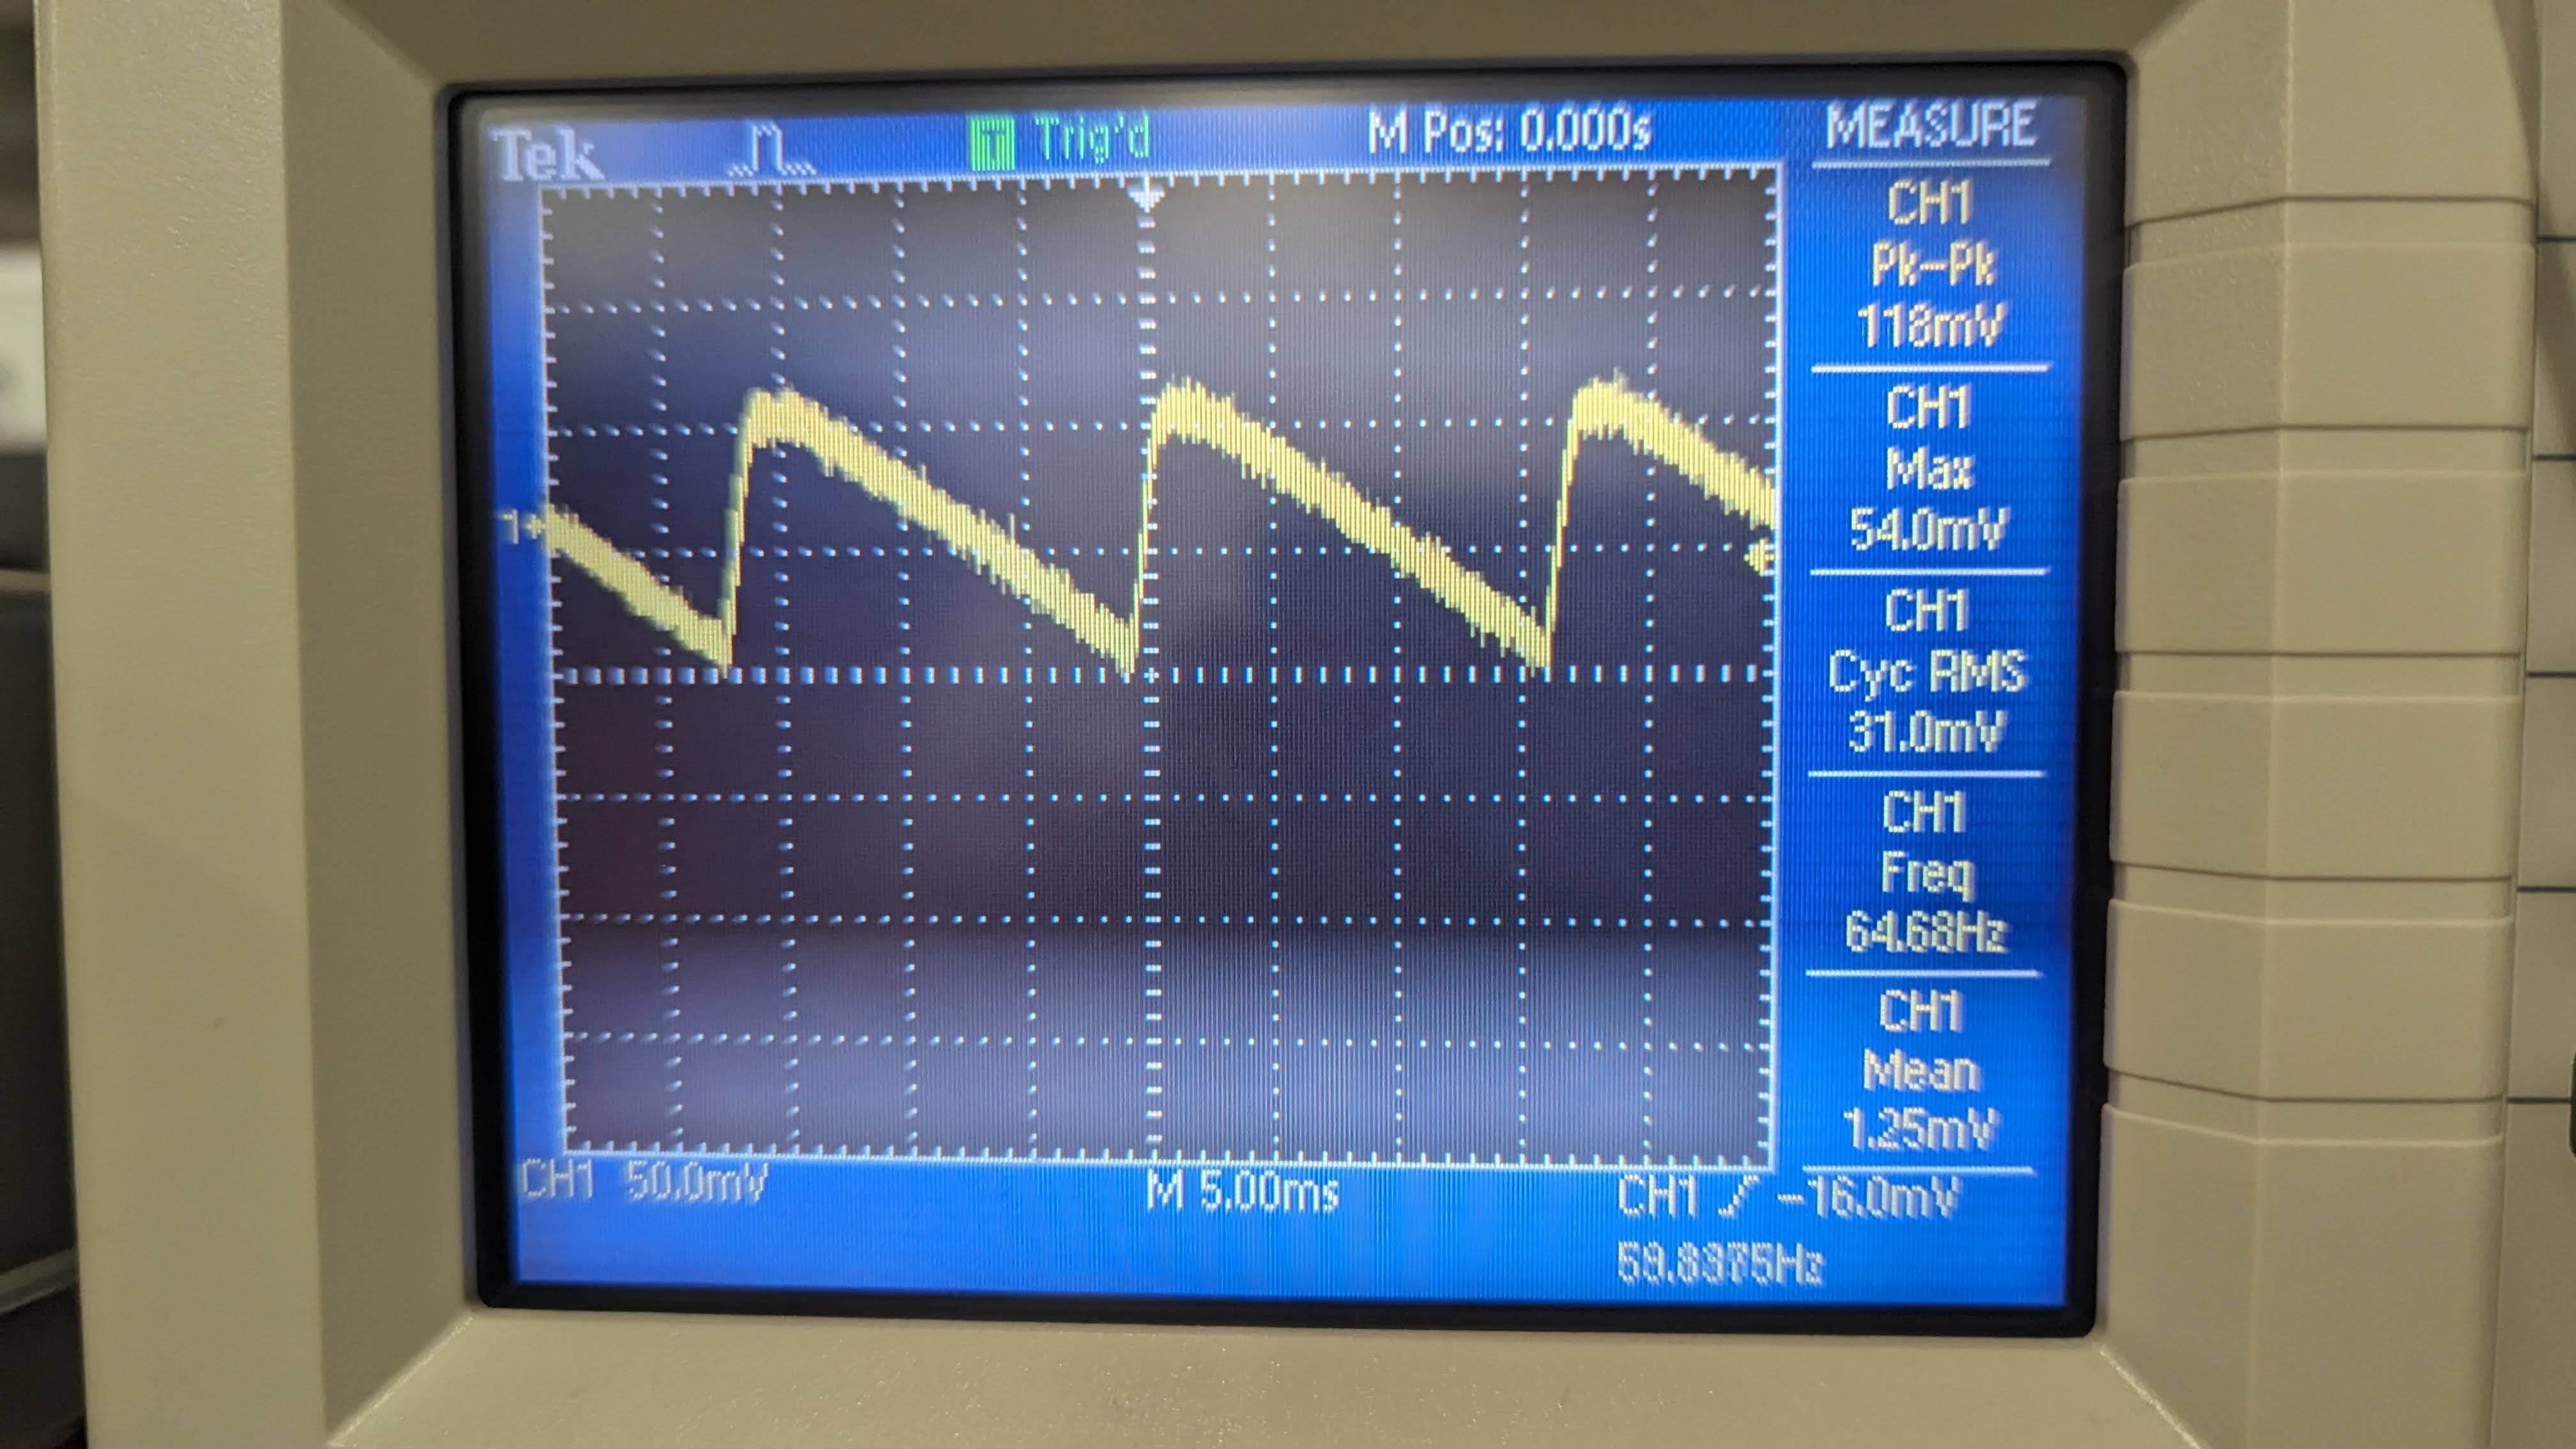
\includegraphics[width=0.45\textwidth]{lab1/t3b}
        \caption{Task 3 waveforms. Left is the DC waveform, while right is the AC coupled component. See the main text for more detailed analysis.}
        \label{fig:t3w}
\end{figure}

\end{document}
